\documentclass[a4paper,14pt]{article}

%%% Работа с русским языком
\usepackage[english,russian]{babel}   %% загружает пакет многоязыковой вёрстки
\usepackage{fontspec}      %% подготавливает загрузку шрифтов Open Type, True Type и др.
\defaultfontfeatures{Ligatures={TeX},Renderer=Basic}  %% свойства шрифтов по умолчанию
\setmainfont[Ligatures={TeX,Historic}]{Times New Roman} %% задаёт основной шрифт документа
\setsansfont{Arial}                    %% задаёт шрифт без засечек
\setmonofont{Courier New}
\usepackage{indentfirst}
\frenchspacing

%%% Дополнительная работа с математикой
\usepackage{amsmath,amsfonts,amssymb,amsthm,mathtools} % AMS
\usepackage{icomma} % "Умная" запятая: $0,2$ --- число, $0, 2$ --- перечисление

\renewcommand{\epsilon}{\ensuremath{\varepsilon}}
\renewcommand{\phi}{\ensuremath{\varphi}}
\renewcommand{\kappa}{\ensuremath{\varkappa}}
\renewcommand{\le}{\ensuremath{\leqslant}}
\renewcommand{\leq}{\ensuremath{\leqslant}}
\renewcommand{\ge}{\ensuremath{\geqslant}}
\renewcommand{\geq}{\ensuremath{\geqslant}}
\renewcommand{\emptyset}{\varnothing}

%%% Работа с картинками
\usepackage{graphicx}  % Для вставки рисунков
\graphicspath{%
	{images/equally-spaced-arrays},
	{images/array-distributions-theory},
	{images/array-distributions-modeling},
	{images/interpolation},
	{images/iterative},
	{images/mimo},
}  % папки с картинками
%\usepackage{subfig}
\setlength\fboxsep{3pt} % Отступ рамки \fbox{} от рисунка
\setlength\fboxrule{1pt} % Толщина линий рамки \fbox{}
\usepackage{wrapfig} % Обтекание рисунков текстом
\usepackage[lflt]{floatflt}
\usepackage{subcaption}
\usepackage[labelfont=bf]{caption}
\captionsetup{justification=centering,singlelinecheck=false}
\renewcommand\thesubfigure{\asbuk{subfigure}}
\counterwithin{figure}{section}
\usepackage{float}

% Работа с графиками
\usepackage{tikz}
\usepackage{pgfplots}
\usepackage{pgfplotstable}

%%% Работа с таблицами
\usepackage{array,tabularx,tabulary,booktabs} % Дополнительная работа с таблицами
\counterwithin{table}{section}
%%%%%%%%%%%%%%%%%%%%%%%%%%%%%%%%%%%%%%%%%%%%%%%%%%%%%%%%%%%%%%%%%%%%%%%%
\usepackage{tabularray}
\DefTblrTemplate{caption-tag}{default}{\textbf{\tablename\hspace{0.25em}\thetable}}
\DefTblrTemplate{caption-sep}{default}{\enskip}
\DefTblrTemplate{caption-text}{default}{\InsertTblrText{caption}}

\DefTblrTemplate{caption}{default}{
	\raggedleft
	\UseTblrTemplate{caption-tag}{default}
	\UseTblrTemplate{caption-sep}{default}
	\UseTblrTemplate{caption-text}{default}

}

\DefTblrTemplate{contfoot-text}{default}{Продолжение на следующей странице}
\SetTblrTemplate{contfoot-text}{default}

\DefTblrTemplate{conthead-text}{default}{(Продолжение)}

\DefTblrTemplate{conthead}{default}{
	\UseTblrTemplate{conthead-text}{default}
}

\DefTblrTemplate{capcont}{default}{
	\hfill
	\UseTblrTemplate{caption-tag}{default}
	\UseTblrTemplate{caption-sep}{default}
	\UseTblrTemplate{caption-text}{default}
	\UseTblrTemplate{conthead-text}{default}
}
%%%%%%%%%%%%%%%%%%%%%%%%%%%%%%%%%%%%%%%%%%%%%%%%%%%%%%%
\usepackage{multirow} % Слияние строк в таблице
\usepackage{array}

%%% Программирование
\usepackage{tcolorbox}
\usepackage{etoolbox} % логические операторы

%%% Страница
\usepackage{extsizes} % Возможность сделать 14-й шрифт
\usepackage{geometry}
\geometry{top=20mm}
\geometry{bottom=20mm}
\geometry{left=30mm}
\geometry{right=15mm}
%%%
\righthyphenmin=2

%%% Настройка отображения содержания
\usepackage{tocloft}
\renewcommand{\cftpartleader}{\cftdotfill{\cftdotsep}} % for parts
\renewcommand{\cftsecleader}{\cftdotfill{\cftdotsep}} % for sections
%%% Заголовки
\usepackage{titlesec}
\titleformat{\section}{\Large\normalfont\bfseries\raggedright}{\arabic{section}.}{0.5ex}{}
\titleformat{\subsection}{\large\normalfont\bfseries\raggedright}{\arabic{section}.\arabic{subsection}.}{0.5ex}{}
\titleformat{\subsubsection}{\normalfont\bfseries\raggedright}{\arabic{section}.\arabic{subsection}.\arabic{subsubsection}.}{0.5ex}{}
\titlespacing*{\section}{0pt}{\baselineskip}{\baselineskip}

\providecommand\phantomsection{}
%\newcommand\schap[1]{\chapter*{#1} \addcontentsline{toc}{chapter}{#1} \phantomsection}
\newcommand\ssect[1]{\section*{#1} \phantomsection \addcontentsline{toc}{section}{#1} \markboth{#1}{#1}}
\newcommand{\rwn}{\the\numexpr\value{rownum}-1\relax}
%%% Custom appendix naming
\usepackage[toc,page]{appendix}
\renewcommand\appendixname{Приложение}
\renewcommand\appendixpagename{Приложения}
\renewcommand\appendixtocname{Приложения}



%%% Ссылки
%\usepackage[superscript]{cite} % Ссылки в верхних индексах
%\usepackage[nocompress]{cite} % 
\usepackage{csquotes} % Еще инструменты для ссылок
%\renewcommand{\refname}{Список источников}
%\addto\captionsrussian{\def\refname{Список источников}}

\usepackage[%
	backend=biber,% движок
	bibencoding=utf8,% кодировка bib файла
	sorting=none,% настройка сортировки списка литературы
	style=gost-numeric,% стиль цитирования и библиографии (по ГОСТ)
	language=autobib,% получение языка из babel/polyglossia, default: autobib % если ставить autocite или auto, то цитаты в тексте с указанием страницы, получат указание страницы на языке оригинала
	autolang=other,% многоязычная библиография
	clearlang=true,% внутренний сброс поля language, если он совпадает с языком из babel/polyglossia
	defernumbers=true,% нумерация проставляется после двух компиляций, зато позволяет выцеплять библиографию по ключевым словам и нумеровать не из большего списка
	sortcites=true,% сортировать номера затекстовых ссылок при цитировании (если в квадратных скобках несколько ссылок, то отображаться будут отсортированно, а не абы как)
	doi=false,% Показывать или нет ссылки на DOI
	isbn=false,% Показывать или нет ISBN, ISSN, ISRN
	mincitenames=3,
	maxcitenames=3,
	maxbibnames=3,
]{biblatex}

\addbibresource{include/references.bib}

\DefineBibliographyStrings{russian}{%
	bibliography = {Список источников},
}

%\renewcommand{\baselinestretch}{1.15}
%\usepackage{setspace} % Интерлиньяж
%\spacing{1.15}
%\onehalfspacing % Интерлиньяж 1.5
%\doublespacing % Интерлиньяж 2
%\singlespacing % Интерлиньяж 1

\usepackage{lastpage} % Узнать, сколько всего страниц в документе.


\usepackage{soul} % Модификаторы начертания
\usepackage{hyperref}
\hypersetup{%
	colorlinks=true,
	linkcolor=blue,
	filecolor=magenta,
	urlcolor=cyan,
	pdfauthor={Лазба Филипп},
	pdftitle={Магистерская диссертация на тему «исследование методов оптимизации современных антенных решеток»},
	pdfsubject={Исследование методов оптимизации современных антенных решеток},
	pdfkeywords={АФАР; ЦАР; AESA; DAA; антенные решётки},
	bookmarks=true,
	pdfpagemode=UseThumbs,
}


%\renewcommand{\familydefault}{\sfdefault} % Начертание шрифта

\usepackage{multicol} % Несколько колонок




\renewcommand{\epsilon}{\ensuremath{\varepsilon}}
\renewcommand{\phi}{\ensuremath{\varphi}}
\renewcommand{\kappa}{\ensuremath{\varkappa}}
\renewcommand{\le}{\ensuremath{\leqslant}}
\renewcommand{\leq}{\ensuremath{\leqslant}}
\renewcommand{\ge}{\ensuremath{\geqslant}}
\renewcommand{\geq}{\ensuremath{\geqslant}}
\renewcommand{\emptyset}{\varnothing}

\newcommand{\bhline}[1]{\noalign{\hrule height #1pt}}



\renewcommand{\theenumii}{\arabic{enumi}.}
\renewcommand{\theenumii}{\arabic{enumi}.\arabic{enumii}}
\renewcommand{\theenumiii}{\arabic{enumi}.\arabic{enumii}.\arabic{enumiii}}

% \usepackage{xassoccnt}
% \NewTotalDocumentCounter{totalfigures}
% \NewTotalDocumentCounter{totaltables}
% \DeclareAssociatedCounters{figure}{totalfigures}
% \DeclareAssociatedCounters{table}{totaltables}

% \usepackage{listings}
% \usepackage{matlab-prettifier}

\usepackage{minted}
\usemintedstyle{friendly_grayscale}
\renewcommand\theFancyVerbLine{\normalsize\arabic{FancyVerbLine}}

%%%%%%%%%%%%%%%%%%%%%%%%%%%%%%%%%%%%%%%%%%%%%%%%%%%%%%%%%%%%%%%

\newcommand*{\figoneendian}{\totalfigures~рисунок}
\newcommand*{\figfourendian}{\totalfigures~рисунка}
\newcommand*{\figfiveendian}{\totalfigures~рисунков}

% Расчёт значений для общего числа рисунков
\newcommand*{\printtotfig}[1][,]{%
	\newbool{less11Q}%
	\newbool{greater19Q}%
	\boolfalse{less11Q}%
	\boolfalse{greater19Q}%
	\newcounter{Ptempnumexpr}%
	\newcounter{Pwordindex}%
	\setcounter{Ptempnumexpr}{0}%
	\addtocounter{Ptempnumexpr}{\numexpr\totalfigures-100*(\totalfigures/100)}%
	\ifnumequal{\totalfigures}{-1}%
	{??#1}%
	{\ifnumequal{\totalfigures}{0}{}%
		{\ifnumless{\value{Ptempnumexpr}}{11}{\booltrue{less11Q}}{}%
			\ifnumgreater{\value{Ptempnumexpr}}{19}{\booltrue{greater19Q}}{}%
			\ifboolexpr{bool {less11Q} or bool {greater19Q}}%
			{\setcounter{Pwordindex}{0}%
				\addtocounter{Pwordindex}{\numexpr\value{Ptempnumexpr}-10*(\value{Ptempnumexpr}/10)}%
				\ifnumequal{\value{Pwordindex}}{1}% Окончание для 1
				{\figoneendian}%
				{\ifnumequal{\value{Pwordindex}}{2}% Окончание для 4
					{\figfourendian}%
					{\ifnumequal{\value{Pwordindex}}{3}%
						{\figfourendian#1}%
						{\ifnumequal{\value{Pwordindex}}{4}%
							{\figfourendian}%
							{\figfiveendian}% Окончание для 5
						}%
					}%
				}%
			}%
			{\figfiveendian}% Окончане для 5
		}%
	}%
}

\usepackage[figure,table]{totalcount}

\author{Лазба Филипп}
\title{}
\date{\today}

\renewcommand{\baselinestretch}{1.15} % put the factor in the second argument 
\usepackage{ragged2e}
\justifying{}

\begin{document}
\thispagestyle{empty}
\setcounter{page}{1}

\begin{center}
    МИНОБРНАУКИ РОССИИ

    \vspace{1ex}

    Федеральное государственное автономное образовательное учреждение 
    
    высшего образования

    \textbf{НАЦИОНАЛЬНЫЙ ИССЛЕДОВАТЕЛЬСКИЙ УНИВЕРСИТЕТ <<МОСКОВСКИЙ ИНСТИТУТ ЭЛЕКТРОННОЙ ТЕХНИКИ>>}

    \vspace{1ex}

    Институт микроприборов и систем управления
\end{center}

\vspace{17ex}

\begin{center}
    Лазба Филипп Борисович 
    
    \vspace{1ex}
    \textbf{Магистреская диссертация}

    по направлению
    \textbf{\textit{11.04.01 <<Радиотехника>>}}
    
    \vspace{1ex}
    \textit{Исследование методов оптимизации современных антенных решеток}

\end{center}

\vspace{25ex}

% \begin{longtblr}[
% 	caption = {Основные параметры SPF5043Z},
% 	label = {table:LNA-parameters}
% 	]{
% 		colspec={Q[1,l,m]Q[1,l,m]},width=\textwidth,
% 		vlines,hlines,
% 		vspan=even,
% 		rowhead=1,
% 		row{1}={font=\bfseries}
% 	}
% 	%%%%%%%%%%%%%%%%%%%%%%%%%%%%%%%%%%%%%%%%%%%%%%%
% 	Параметр & Значение \\
% 	%%%%%%%%%%%%%%%%%%%%%%%%%%%%%%%%%%%%%%%%%%%%%%%%
% 	Усиление & 18,2 дБ \\
% 	Коэффициент шума & 0,7 дБ \\
% 	Точка однодецибельной компрессии & 22,6 дБмВт \\
% 	Размеры ШхДхВ & 2х2х1 мм \\
% \end{longtblr}

\SetTblrTemplate{caption}{empty}

\begin{longtblr}[
  ]{
    colspec = {Q[l] Q[c] Q[r]},
    row{odd} = {m},
    row{even} = {m}
  }
  Студент   & \SetCell[r=1]{c}\underline{\hspace{5cm}} & Лазба Ф.Б. \\
  Руководитель   & & \\
  к.т.н., доцент & \SetCell[r=1]{c}\underline{\hspace{5cm}} & Орешкин В.И. \\
            & & \\
\end{longtblr}

\SetTblrTemplate{caption}{default}

\vfill

\begin{center}
    Москва, Зеленоград

    2024
\end{center}

\newpage

{\Large\normalfont\bfseries \hfil Аннотация}
\vspace{1em}
\thispagestyle{empty}

Магистерская диссертация на тему «исследование методов оптимизации современных антенных решеток».

Работа состоит из введения, 5 глав, заключения, списка источников и приложений.

В работе рассмотрены существующие подходы к решению задач оптимизации антенных решёток и 
особенности их реализации; проведено моделирование, на основе которого были сделаны выводы.

В заключении приведены выводы и итог проведённого исследования.

Работа содержит~\pageref*{LastPage} страниц, 2~таблицы, \printtotfig.
Для написания данной работы было использовано 33 источника. 

\ 

{\Large\normalfont\bfseries \hfil Annotation}
\vspace{1em}
\thispagestyle{empty}

Master's thesis on the topic "research of optimization methods for modern antenna arrays".

The work consists of an introduction, 5 chapters, a conclusion, a list of sources and appendices.

The paper considers existing approaches to solving antenna array optimization problems and the features of
their implementation; modeling is carried out, on the basis of which conclusions were drawn.

In conclusion, results of the study are presented.

The work contains~\pageref*{LastPage} pages, 2~tables, \totalfigures~figures. 
A total of 33 sources were used to write this work.

\tableofcontents{}
\ssect{Список терминов и сокращений}

{
\noindent \textbf{АР} --- антенная решётка

\noindent \textbf{ФАР} --- фазированная антенная решётка

\noindent \textbf{АФАР} --- активная фазированная антенная решётка

\noindent \textbf{РНС} --- радионавигационная система

\noindent \textbf{ЦАР} --- цифровая антенная решётка

\noindent \textbf{ДН} --- диаграмма направленности

\noindent \textbf{ДНА} --- диаграмма направленности антенны

\noindent \textbf{УБЛ} --- уровень боковых лепестков

\noindent \textbf{УДЛ} --- уровень дифракционных лепестков

\noindent \textbf{ШГЛ} --- ширина главного лепестка
}
\ssect{Введение}\label{chap:introduction}

Антенные решётки играют важную роль во многих сферах современной жизни. Их применение можно увидеть, например, в следующих областях:

\begin{itemize}
      \item Системы радиосвязи
            \begin{itemize}
                  \item В базовых станциях мобильной связи для создания узких областей покрытия, что помогает
                        обеспечивать связь в труднодоступных зонах и осуществлять пространственное
                        разделение в густонаселенных районах, что позволяет увеличить пропускную способность
                  \item В системах спутниковой связи для осуществления покрытия сигналом больших областей
                        и улучшения качества связи за счёт создания узких, но быстро перестраиваемых диаграмм направленности.
            \end{itemize}
      \item Радиолокационные системы
            \begin{itemize}
                  \item Применение антенных решёток в военных, авиационных и автомобильных радарах позволяет быстро сканировать пространство
                        и эффективно обнаруживать объекты и вычислять их параметры (местоположение, скорость и направление движения);
                        осуществлять слежение за быстро передвигающимися целями и принимать решения на основе полученных данных.
            \end{itemize}
      \item Радиоастрономия
            \begin{itemize}
                  \item В радиотелескопах, таких как Very Large Array (VLA), для изучения космических
                        радиоволн, исходящих от различных астрономических объектов.
            \end{itemize}
\end{itemize}

Несмотря на свои многочисленные достоинства, активные фазированные антенные решётки обладают такими недостатками
как сложность разработки, возможные большие размеры и высокая стоимость. В зависимости от области применения инженерам
приходится находить оптимальные соотношения между сложностью, стоимостью, скоростью сканирования, размерами, ремонтопригодностью
и многими другими параметрами антенных решёток, которые противоречат друг другу. Ввиду большого количества учитываемых параметров,
многокритериальная оптимизация требует комплексного подхода и глубокого понимания взаимодействия между ними.


Цель данной магистерской работы заключается в проведении обзора существующих методов оптимизации антенных решёток с последующим анализом и сравнением их эффективности.

Задачами данной работы являются:

\begin{itemize}
      \item Исследовать различные геометрические и амплитудно-фазовые распределения
      \item Исследовать метод итеративной обработки данных
      \item Исследовать возможности применения интерполяции в антенных решётках
      \item Исследовать применения технологии MIMO в радиолокаторах
\end{itemize}

Работа направлена на исследование того, как различные методы оптимизации могут влиять на важные параметры системы - такие как сложность, стоимость,
размер и скорость сканирования. На основе проведённого анализа будет сформулирован ряд рекомендаций по выбору и
применению методов в зависимости от специфики задачи и условий эксплуатации.
\section{Литературный обзор}\label{sect:review}
\subsection{Эквидистантные антенные решётки с равномерным распределением амплитуд}\label{subsect:equally-spaced-arrays}

Основополагающие принципы фазированных антенных решёток были заложены ещё в 1905 году Карлом Фердинандом Брауном, который получил Нобелевскую премию 
по физике за разработку методов управления направленностью антенн с помощью фазового сдвига. Однако широкое применение и разработка этих антенн начались 
только в середине 20-го века. Технология начала активно развиваться в 1950-1960х годах в рамках военных и аэрокосмических программ. Первые практические 
применения антенных решёток были связаны с задачами локации и отслеживания воздушных и космических объектов.

Классические ФАР представляют собой массив антенных элементов с одинаковыми характеристиками, расположенными равномерно
на отрезке прямой либо на плоскости. Принцип ФАР заключается в управлении фазами волн в каналах таким образом,
чтобы через синфазное сложение этих волн достигалось усиление принятого сигнала лишь в определённом направлении. 

На Рисунке~\ref{fig:equally-spaced-distribution-pos} показано расположение элементов в линейной антенной решётке. 
Рисунки~\ref{fig:equally-spaced-distribution-beam-pattern0}~-~\ref{fig:equally-spaced-distribution-beam-pattern30} 
отображают диаграммы направленности этой решётки в различных направлениях.



\begin{figure}[!ht]
    \centering
    
\includegraphics[width=0.8\textwidth]{equally-spaced-distribution}
    \caption{Расположение элементов в эквидистантной АР}
    \label{fig:equally-spaced-distribution-pos}
\end{figure}



\begin{figure}[!ht]
    \centering
    \begin{subfigure}[b]{0.55\textwidth}
        \centering
        \hspace*{-3.5ex}
        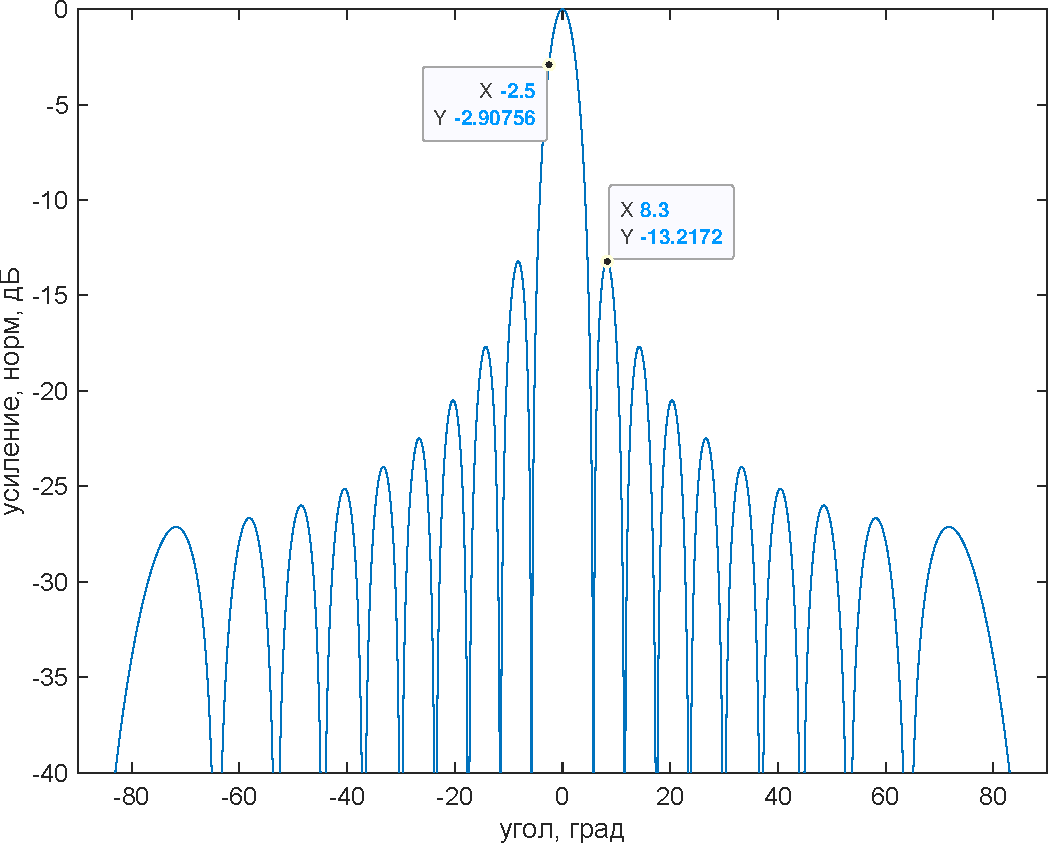
\includegraphics[width=\textwidth]{equally-spaced-distribution-beam-pattern0}
        \caption{}%
        \label{fig:equally-spaced-distribution-beam-pattern0}
    \end{subfigure}
    \hfill
    \begin{subfigure}[b]{0.49\textwidth}
        \centering
        \hspace*{-3ex}
        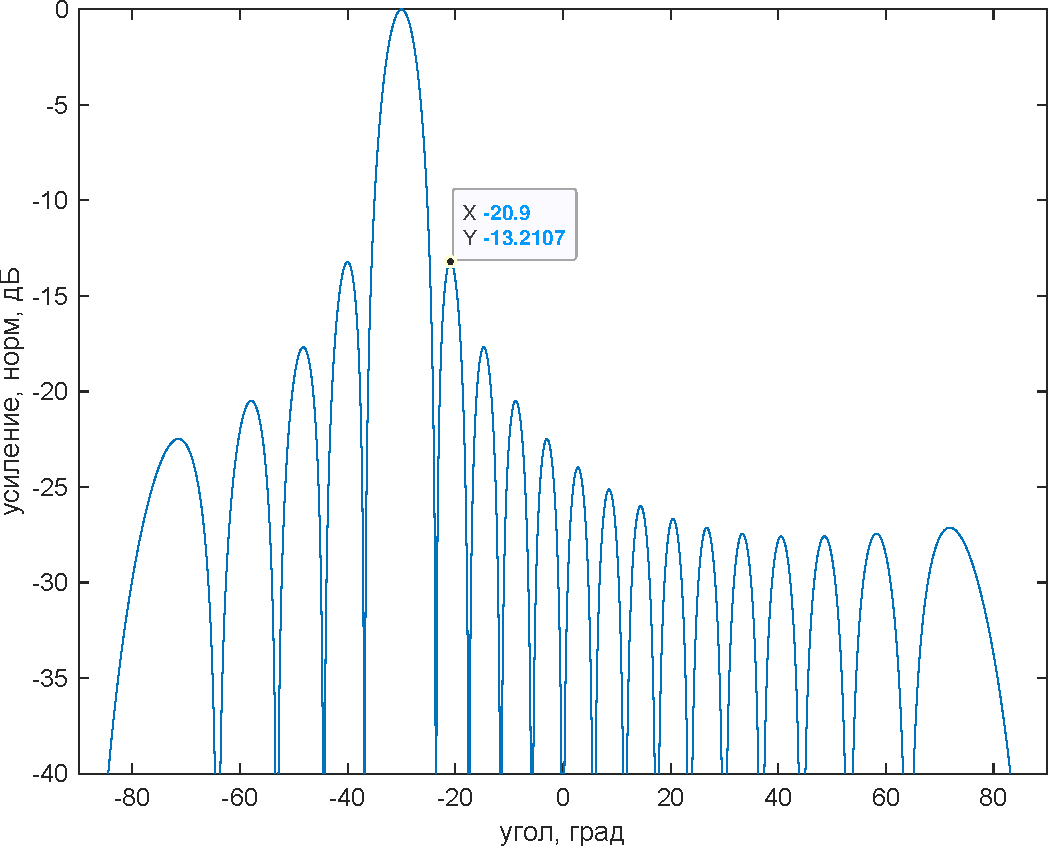
\includegraphics[width=\textwidth]{equally-spaced-distribution-beam-pattern-30}
        \caption{}%
        \label{fig:equally-spaced-distribution-beam-pattern-30}
    \end{subfigure}
    \begin{subfigure}[b]{0.49\textwidth}
        \centering
        \hspace*{-3ex}
        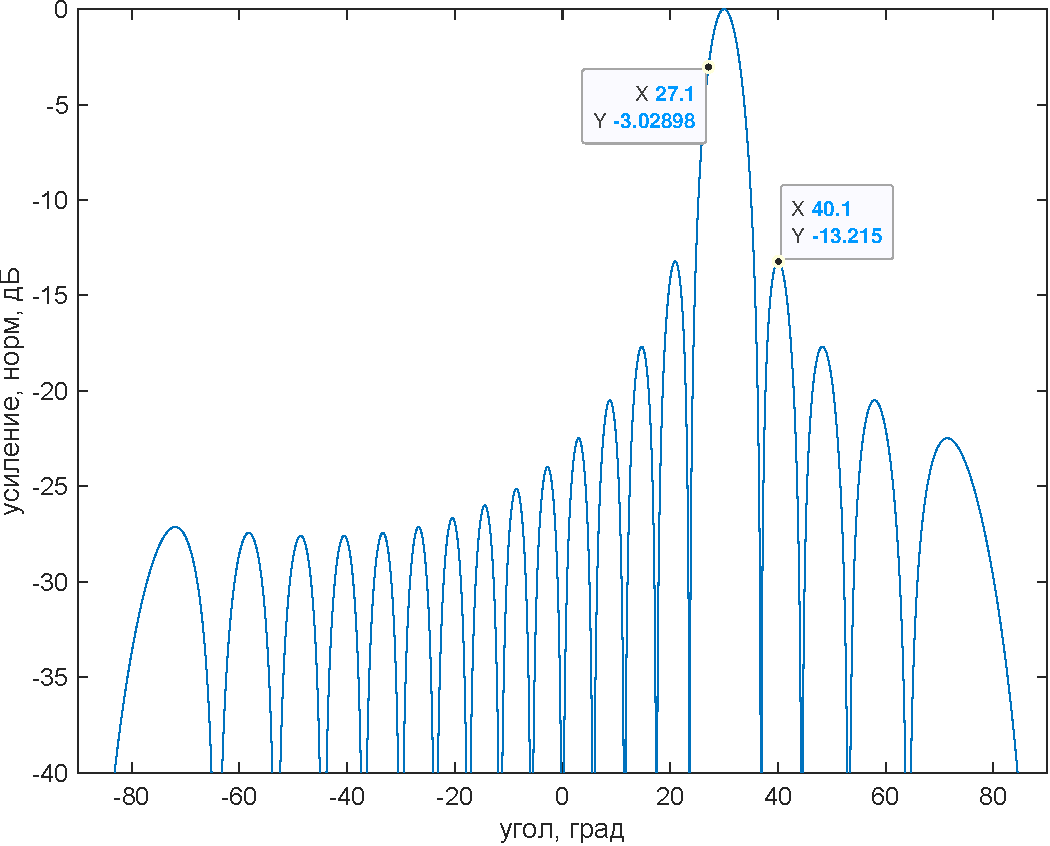
\includegraphics[width=\textwidth]{equally-spaced-distribution-beam-pattern30}
        \caption{}%
        \label{fig:equally-spaced-distribution-beam-pattern30}
    \end{subfigure}
    \caption{%
        ДН при отклонении луча на
        (а) 0
        (б) -30 и
        (в) +30 градусов
    }%
    \label{fig:equally-spaced-distribution}
\end{figure}

Такие антенные решётки применяются и в современных устройствах ввиду простоты их проектирования, 
однако они имеют несколько недостатков: высокий уровень боковых лепестков 
(на Рисунке~\ref{fig:equally-spaced-distribution} видно, что уровень второго лепестка составляет порядка -13 дБ от основного) 
и высокая стоимость из-за большого количества элементов, которое необходимо для поддержания требуемой
ширины основного лепестка при расстоянии между элементами $d \leq \lambda/2$. 
Увеличение же межэлементного расстояния приводит к появлению дифракционных 
лепестков (ложных целей), пример такого явления можно увидеть на Рисунке \ref{fig:equally-spaced-distribution-granting-lobes}.

\begin{figure}[!ht]
    \centering
    \hspace*{-3ex}
    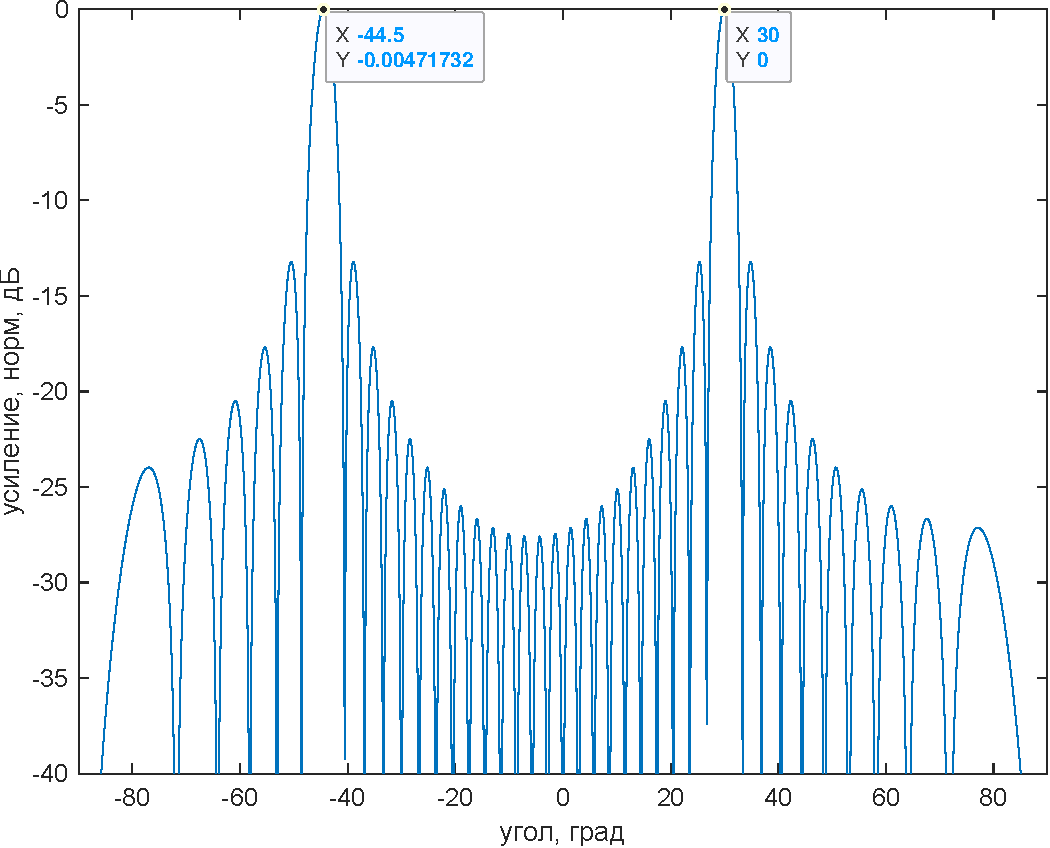
\includegraphics[width=0.8\textwidth,height=0.35\textheight,keepaspectratio]{equally-spaced-distribution-granting-lobes}
    \caption{ДН при межэлементном расстоянии $d > \lambda/2$,
        направленность на~20~градусов,
        дифракционный лепесток~на~-44,5~градусов}%
    \label{fig:equally-spaced-distribution-granting-lobes}
\end{figure}

Потому такие решётки применяются в системах, где отсутствие множественной направленности менее критично, 
чем увеличение размера/веса итогового устройства, например, в системах межспутниковой связи. 
Кроме того, важную роль играет простота изготовления и наладки таких ФАР.

В системах, где параметры направленности являются критичными, а также в тех случаях когда 
есть возможность применять более сложные подходы, используются решётки, разработанные с помощью методов, 
которые будут описаны в следующих разделах данной работы. 


\subsection{Неэквидистантные антенные решётки и неравномерные амплитудные распределения}\label{sect:distributions-theory}


Классическим подходом к оптимизации антенных решёток является применение различных амплитудных и геометрических
распределений \cite{harrington1961sidelobe, ma1963note, brown1962note}.Под оптимизацией понимается уменьшение
количества антенных элементов при сохранении заданнойширины главного лепестка и поддержания низкого уровня
боковых и дифракционных лепестков диаграммы направленности, либо улучшение
характеристик ДНА при том же либо меньшем количестве элементов.
Целью методов, которые применяют такой подход является нахождение таких амплитудных распределений и положений
антенных элементов при которых будут достигнуты наилучшие характеристики диаграммы направленности при
заданном максимальном количестве каналов антенной решётки. Методы этой группы включают в себя ручную
оптимизацию на основе изначально выбранного распределения \cite{lyalin2019, kuzmin2019ring, andreasen1962linear};
поиск математических приближений \cite{ishimaru1962theory, harrington1961sidelobe};
применение итеративных функций поиска (LMS алгоритм)\cite{ma1997weighted} и вероятностных методов,
таких как генетические деревья, муравьиный алгоритм, метод роя частиц и другие.
\cite{jain2012solving, dubey2023cosecant, luo2015synthesis}.

\subsubsection{Ручная оптимизация}\label{sec:manual-optimization}

Одним из применяемых подходов заключается в выборе изначального распределения и дальнейшее его изменение
на основе некоторых гипотез о влиянии тех или иных изменений на итоговую диаграмму и в
соответствии с результатами проведённого моделирования.

В качестве примера можно привести работы \cite{lyalin2019, kuzmin2019ring}, в которых в качестве
изначального распределения выбрана кольцевая концентрическая антенная решётка, в которой элементы
расположены группами прямоугольных элементов, которые в свою очередь расположены на нескольких
концентрических кольцах. Меняя угол поворота прямоугольных групп, а также смещая по фазе концентрические
окружности, можно найти некоторое расположение, удовлетворяющее техническому заданию.
Результат такой оптимизации показан на Рисунках~\ref{fig:manual-opt-pos},~\ref{fig:manual-opt-radiation-pattern}.
Видно, что уровень боковых лепестков соответствует эквидистантной решётке, а уровень
дифракционных лепестков не превышает УБЛ. При этом число антенных элементов
значительно меньше чем в эквидистантной решётке с межэлементным расстоянием $d \leq \lambda/2$ и полным заполнением апертуры.

\begin{figure}[H]
    \centering
    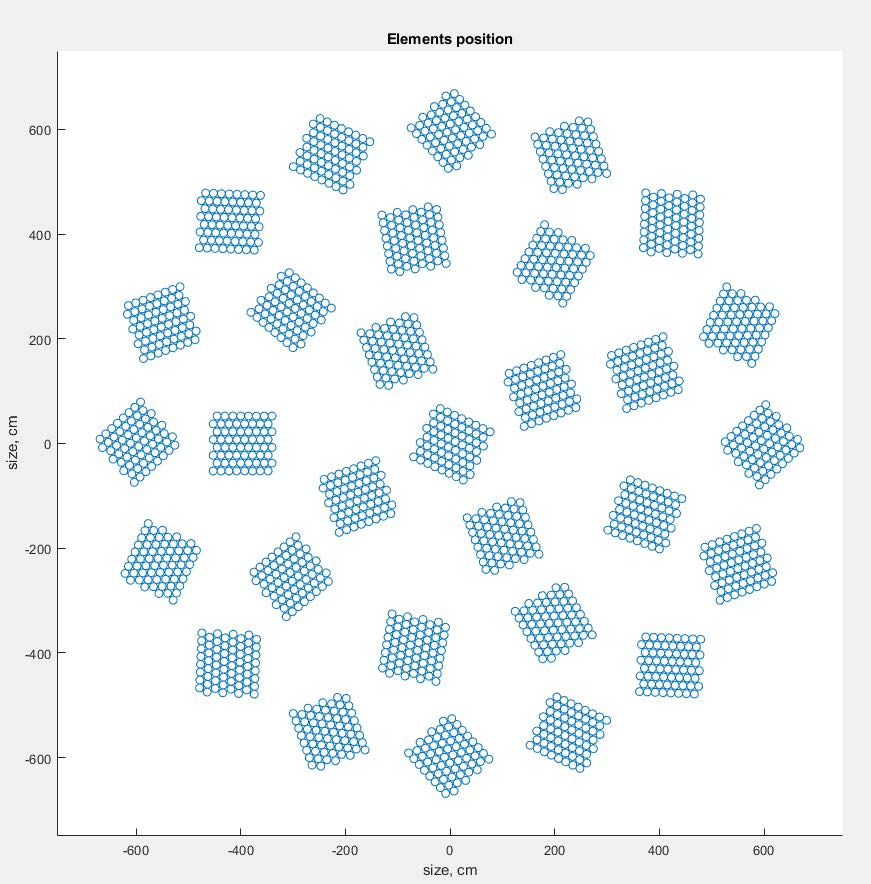
\includegraphics[width=0.8\textwidth,height=0.35\textheight,keepaspectratio]{manual-opt-pos}
    \caption{Итоговое расположение элементов}%
    \label{fig:manual-opt-pos}
\end{figure}


\begin{figure}[H]
    \centering
    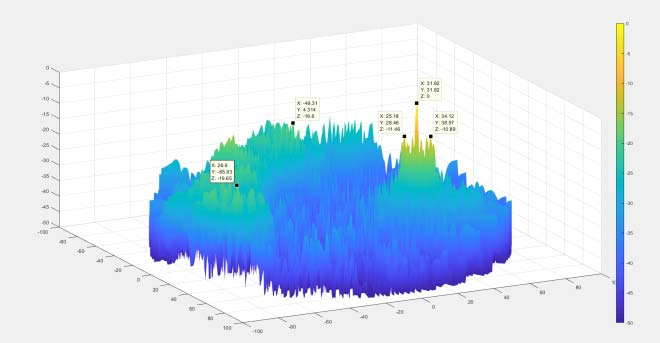
\includegraphics[width=0.8\textwidth,height=0.35\textheight,keepaspectratio]{manual-opt-radiation-pattern}
    \caption{Диаграмма направленности с отклонением на 30 градусов по углам~$\theta$~и~$\phi$. УБЛ~-11~дБ, УДЛ~-19~$\div$~-12~дБ}%
    \label{fig:manual-opt-radiation-pattern}
\end{figure}


\subsubsection{Неравномерные амплитудные распределения}\label{sect:amplitude-distributions}

Известно, что спадающие к краям амплитудные распределения позволяют уменьшить уровень боковых
лепестков при некотором расширении главного лепестка \cite{schelkunoff1943mathematical}.
Например, в работе \cite{schelkunoff1943mathematical} показно уменьшение уровня боковых
лепестков относительно решётки с равноамплитудным распределением при
использовании равномерно спадающей к краям амплитуды.

\begin{figure}[H]
    \centering
    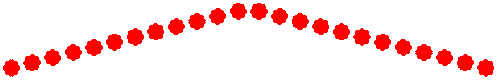
\includegraphics[width=0.8\textwidth,height=0.35\textheight,keepaspectratio]{linear-decreasing-distribution}
    \caption{Пример равномерно спадающего к краям амплитудного распределения}%
    \label{fig:linear-decreasing-distribution}
\end{figure}

Позже были рассмотрены и другие распределения похожего вида. Так, распределение вида “косинус на пьедестале”
(Рисунок~\ref{fig:partial-sum-method}), выводимое с помощью метода парциальных ДН, позволяет
проводить расчёт усилений в каналах антенной решётки по некоторым заданным характеристикам
диаграммы направленности. \cite{Chist2012}

\begin{figure}[H]
    \centering
    \begin{subfigure}[b]{0.4\textwidth}
        \centering
        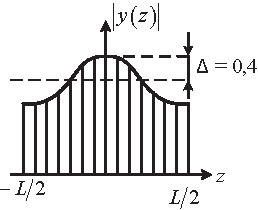
\includegraphics[width=\textwidth,height=0.35\textheight,keepaspectratio]{partial-sum-distribution}
        \caption{}%
        \label{fig:partial-sum-distribution}
    \end{subfigure}
    \begin{subfigure}[b]{0.4\textwidth}
        \centering
        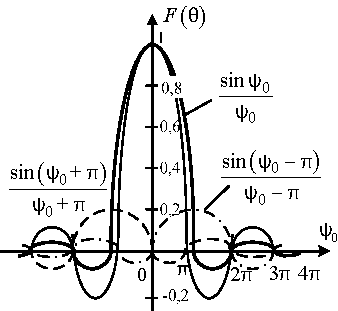
\includegraphics[width=\textwidth,height=0.35\textheight,keepaspectratio]{partial-sum-pattern}
        \caption{}%
        \label{fig:partial-sum-pattern}
    \end{subfigure}
    \caption{%
        Распределение вида “косинус на пьедестале” и соответствующая ему ДНА
    }%
    \label{fig:partial-sum-method}
\end{figure}

В зарубежной литературе классическим подходом считается применение оконных функций Дольфа-Чебышева
\cite{andreasen1962linear, harrington1961sidelobe, jain2012solving, luo2015synthesis, subbarao2015tapering, ishimaru1962theory}.

Распределение было предложено Ч. Дольфом в 1946 году \cite{dolph1946current}.
Данный метод позволяет значительно уменьшить максимальный уровень боковых
лепестков за счёт увеличения среднего УБЛ и небольшого расширения
основного лепестка. Данный способ обладает следующими преимуществами \cite{vendik2018antenna}:

\begin{enumerate}
    \item УБЛ одинаков для всех лепестков
    \item Положение боковых лепестков диаграммы направленности определяется расчётом
    \item Распределение позволяет обеспечить заданную ширину луча
\end{enumerate}

Многочлены Чебышева имеют следующий вид:

\begin{equation*}
    T_n(x)=\cos{\left[n \cdot \arccos{(x)}\right]}
\end{equation*}

Введём параметр:

\begin{equation*}
    u=\frac{2\pi d}{\lambda}\cdot \sin{\theta}
\end{equation*}

И приведём многочлены к следующему виду

\begin{equation}\label{eqn:tcheby-final}
    F(u)=\cos{\left[M\arccos{(z_0 \cdot \cos{(u\cdot z_1)})}\right]}
\end{equation}

здесь $M$ -- число элементов АР, $z_0$ -- высота и $z_1$ -- ширина главного лепестка ДНА.

Формула (\ref{eqn:tcheby-final}) определяет амплитуды.

\begin{figure}[H]
    \centering
    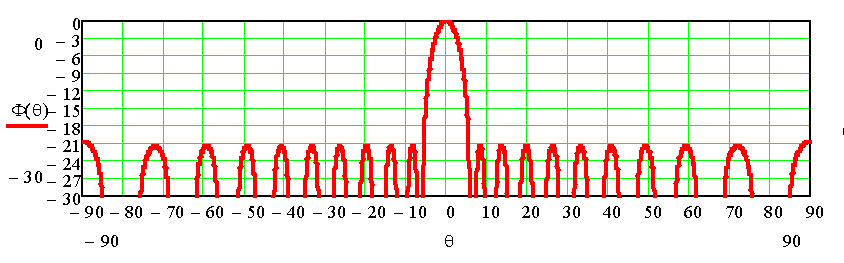
\includegraphics[width=0.8\textwidth,height=0.35\textheight,keepaspectratio]{dolph-tcheby-pattern-review}
    \caption{Диаграмма направленности антенной решётки с окном Дольфа-Чебышева \cite{vendik2018antenna}}%
    \label{fig:dolph-tcheby-pattern-review}
\end{figure}

Другими вариантами оконных функция являются также, например, оконные функции Кайзера и Блэкмана.


\subsubsection{Метод возмущений}\label{sec:perturbations-method}

Метод возмущений, представляет диаграмму направленности антенной решётки в виде суммы
парциальных диаграмм направленности, где каждый член суммы соответствует некоторому
амплитудно-фазовому распределению на элементах АР.
Сумма этих распределений даёт распределение, которое установлено в исследуемой антенной решётке.

В работе \cite{harrington1961sidelobe} рассматрено применение метода возмущений
для поиска смещений положений антенных элементов, при которых будет получена
ДНА с меньшим уровнем боковых лепестков.

Предлагается использовать расширяющееся к краям геометрическое распределение антенных элементов.
Полученное распределение сравнивается с эквидистантной решёткой с амплитудным распределением
Дольфа-Чебышёва. В Таблице~\ref{table:perturbations-pos} и на Рисунке~\ref{fig:perturbation-position-compare} приведены параметры антенной решётки, показанной в статье

\begin{table}[H]
    \resizebox{\textwidth}{!}{%
        \begin{tabular}{c|c|c|c|c|c|c|c|c|c|c|c|c}
            n            & 1      & 3      & 5      & 7      & 9      & 11     & 13     & 15     & 17     & 19     & 21     & 23     \\ \hline
            $\epsilon_n$ & -0,048 & -0,176 & -0,354 & -0,518 & -0,603 & -0,616 & -0,622 & -0,541 & -0,328 & +0,153 & +0,780 & +1,253 \\
        \end{tabular}
    }
    \caption{Относительные смещения элементов}\label{table:perturbations-pos}
\end{table}

\begin{figure}[H]
    \centering
    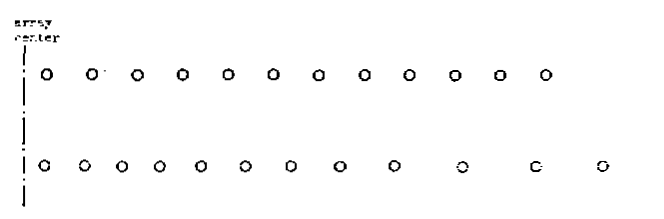
\includegraphics[width=0.8\textwidth,height=0.1\textheight,keepaspectratio]{perturbation-position-compare}
    \caption{Иллюстрация сравнения положений элементов в эквидистантной и исследуемой АР}%
    \label{fig:perturbation-position-compare}
\end{figure}

На Рисунке~\ref{fig:perturbations-radial-pattern} приведены ДНА антенн исследуемой и эталонной.

\begin{figure}[H]
    \centering
    \begin{subfigure}[b]{0.4\textwidth}
        \centering
        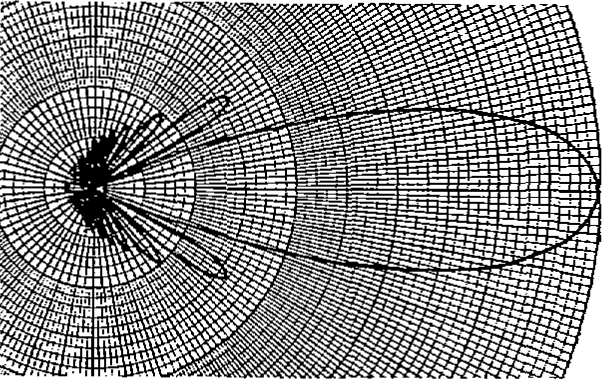
\includegraphics[width=\textwidth,height=0.35\textheight,keepaspectratio]{perturbations-radial-pattern-equidist}
        \caption{}%
    \end{subfigure}
    \begin{subfigure}[b]{0.4\textwidth}
        \centering
        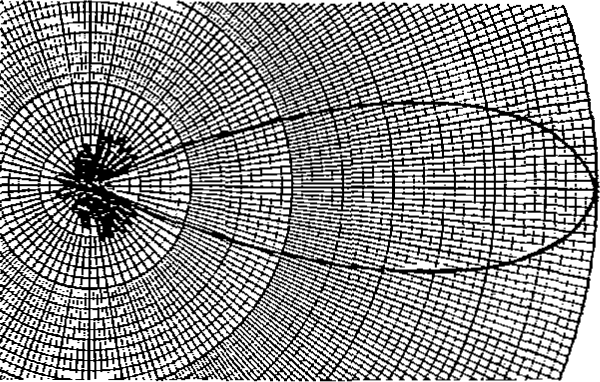
\includegraphics[width=\textwidth,height=0.35\textheight,keepaspectratio]{perturbations-radial-pattern-designed}
        \caption{}%
    \end{subfigure}
    \caption{%
        ДНА
        (а) эквидистантной и
        (б) неэквидистантной антенных решёток
        с одинаковым количеством антенных элементов.
    }%
    \label{fig:perturbations-radial-pattern}
\end{figure}

\begin{sloppypar}
    В статье, однако, отмечено, что уменьшение усиления в области ${0<u<\pi}$ ($u$ - угол от нормали к плоскости АР) приводит к
    увеличению усиления в области ${\pi<u<2\pi}$, т.е. к увеличению дифракционных лепестков, что показано на
    Рисунке~\ref{fig:perturbations-linear-pattern}. Однако это увеличение наблюдается в той области, где усиление, вызванное
    множителем решётки зачастую нивелируется уменьшением усиления множителем
    антенного элемента, что можно наблюдать на {Рисунке~\ref{fig:perturbations-radial-pattern}}.
\end{sloppypar}


\begin{figure}[H]
    \centering
    \begin{subfigure}[b]{0.4\textwidth}
        \centering
        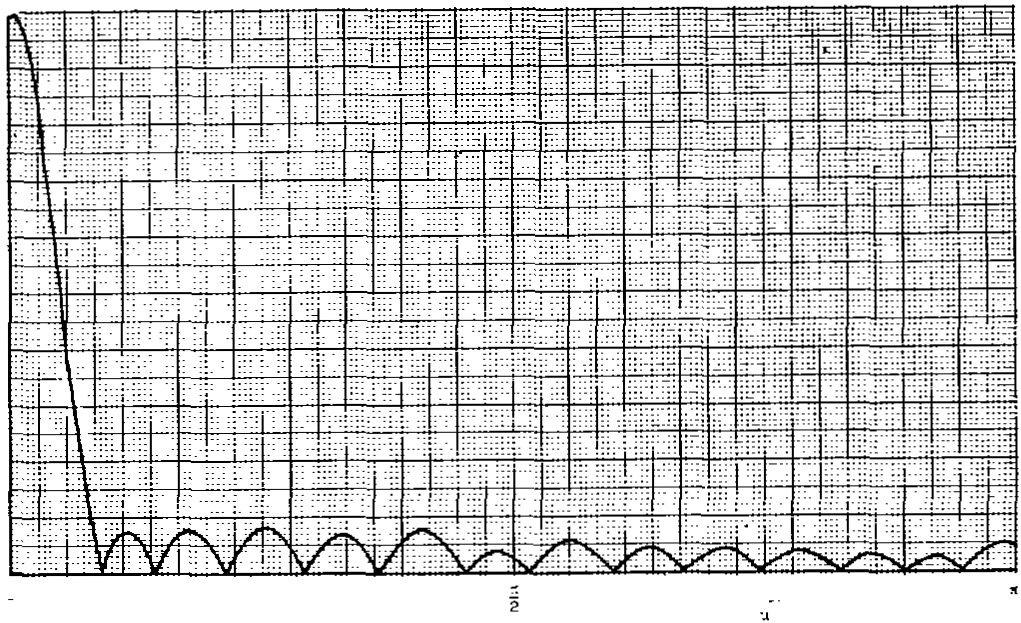
\includegraphics[width=\textwidth,height=0.35\textheight,keepaspectratio]{perturbations-linear-pattern-0pi}
        \caption{}%
    \end{subfigure}
    \begin{subfigure}[b]{0.4\textwidth}
        \centering
        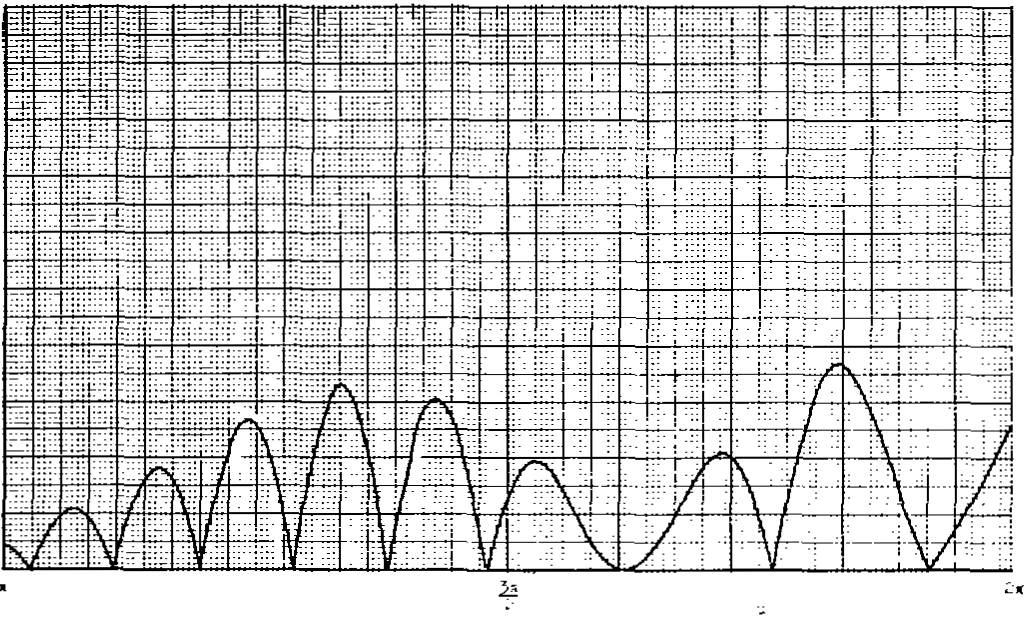
\includegraphics[width=\textwidth,height=0.35\textheight,keepaspectratio]{perturbations-linear-pattern-pi2pi}
        \caption{}%
    \end{subfigure}
    \caption{%
        ДНА при угле сканирования
        (а) от $0$ до $\pi$ и
        (б) от $\pi$ до $2\pi$
    }%
    \label{fig:perturbations-linear-pattern}
\end{figure}

Таким образом, в статье показан метод, при котором можно уменьшить УБЛ за счёт увеличения УДЛ.
При этом преимущества данного метода по сравнению с методом амплитудных распределений следующие:

\begin{itemize}
    \item не расширяется главный лепесток
    \item нет необходимости проектировать АФАР с различным усилениес в каналах, что упрощает разработку
          и удешевляет устройство
    \item больше усиление при равном количестве элементов
\end{itemize}


\subsubsection{Ряды Пуассона}\label{sec:poisson-sum}

Данный метод описан в статье \cite{ishimaru1962theory}. Здесь вводится т.н. функция положения источника,
а диаграмма направленности антенной решётки с неравномерным расположением элементов представляется в виде сумм
Пуассона ДН от множества интегральных (непрерывных) распределений элементов.
Диаграмма направленности АР описывается следующим уравнением

\begin{equation*}
    E(\theta) = \sum_{n=1}^{N} I_n e^{jks_n \sin{\theta}}
\end{equation*}

Используя формулу сумм Пуассона можно привести её к следующему виду:

\begin{equation*}
    E(\theta) = \sum_{n=-\infty}^{\infty} \int_{0}^{N} {f(\nu) e^{j2m\pi\nu} d\nu}
\end{equation*}

Далее вводится функция положения, которая связывает номер элемента с его отступом от края решётки

\begin{figure}[H]
    \centering
    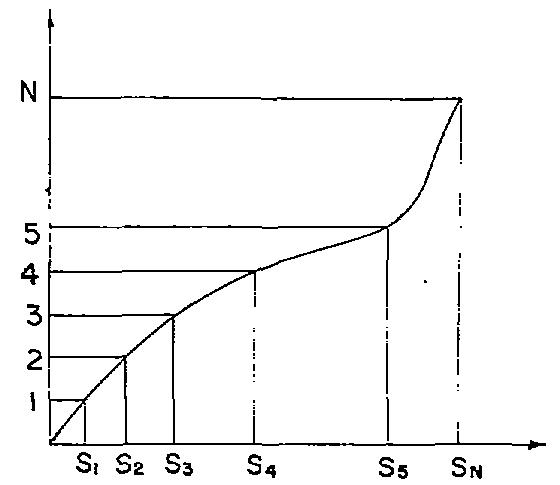
\includegraphics[width=0.8\textwidth,height=0.25\textheight,keepaspectratio]{source-position-function}
    \caption{График функции положения источника}%
    \label{fig:source-position-function}
\end{figure}

Заменив переменную перейдём к следующей формуле

\begin{equation*}
    E(\theta) = \sum_{n=-\infty}^{\infty} E_m(\theta)
\end{equation*}

\begin{equation*}
    E_m(\theta) = \int_{s_0}^{s_N} {A(s) \frac{d\nu}{ds} e^{-j(\xi(s)-2m\pi\nu(s))} e^{jks\sin\theta} ds}
\end{equation*}

Где $A(s)$ описывает амплитуду тока в решётке, причем $A(s)=A_n$ (току в $n$ элементе АР), когда $s=s_n$.

Данная сумма быстро сходится, и потому для вычисления ДН с некоторой погрешностью достаточно будет взять лишь
несколько членов этой последовательности. Так, в примере, показанном в статье, используется лишь
один член последовательности.

\begin{figure}[H]
    \centering
    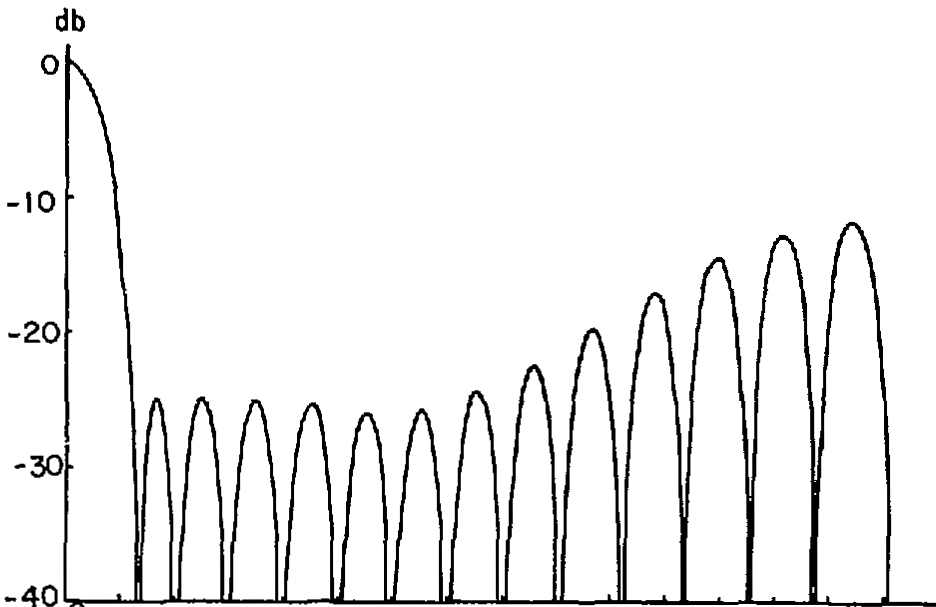
\includegraphics[width=0.8\textwidth,height=0.3\textheight,keepaspectratio]{ishimaru-20el-pattern}
    \caption{ДН антенной решётки из 20 элементов. Полученный УБЛ равен~$-25$~дБ}%
    \label{fig:ishimaru-20el-pattern}
\end{figure}

Достоинства и недостатки данного метода такие же как у метода возмущений,
рассмотренного в подразделе~\ref{sec:perturbations-method}, однако распределение, полученное в статье
\cite{ishimaru1962theory}, имеет меньший уровень усиления вне главного лепестка,
чем распределение из статьи \cite{harrington1961sidelobe}.

\subsubsection{LMS алгоритм}\label{sec:lms-algorithm}

В статье "Weighted Least Square method for Optimum Thinned Antenna Arrays" авторы Xinyu Ma и Byong Kun Chang
рассматривают проблему оптимизации антенных решёток, используя взвешенный метод наименьших квадратов. Основная
задача, решаемая в статье, заключается в нахождении оптимальных межэлементных расстояний в разреженных (thinned)
антенных решётках для получения желаемых характеристик при заданном количестве элементов.

Процесс нахождения наиболее подходящих межэлементных расстояний следующий:
\begin{sloppypar}
    \begin{enumerate}
        \item Определение функции ошибки

              $$
                  E^k (\omega) = W(\omega)\left[H_d(\omega)-H_l^k (\omega)\right]
              $$

              здесь $H_l^k$ -- ДН на k-той итерации, $H_d$ -- эталонная ДН, а $W(\omega)$ -- взвешивающая функция.

              Тогда итоговая ошибка рассчитывается как интегральных

              $$
                  \epsilon^k = \frac{1}{2} \int_{0}^{\pi}{ \left| E^k(\omega) \right|^2 d\omega}
              $$

        \item Итеративное обновление параметров

              Ошибка $\epsilon^k$ может быть аппроксимирована как квадратичная функция от изменений межэлементных расстояний
              $\Delta D_n$. На каждом шаге изменение расстояний рассчитывается как

              $$
                  \Delta D_{n}^{k+1}-\mu \frac{\partial \epsilon^k}{\partial \Delta D_n^k},\ 1\leq n \leq N_l
              $$

              здесь $\mu$--шаг сходимости ДЬЫ алгоритма, $\Delta D_n^k$ и $\Delta D_n^{k+1}$ -- изменения межэлементных расстояний на {k-том} и {k+1-ом} шаге алгоритма, а $\frac{\partial \epsilon^k}{\partial \Delta D_n^k}$~--~градиент-вектор квадрата ошибки.

              Межэлементное расстояние получается как

              $$
                  D_{n}^{k+1} = \Delta D_{n}^{k} + \Delta D_{n}^{k+1}, \ 1\leq n \leq N_l - 1
              $$

    \end{enumerate}
\end{sloppypar}

Функция взвешивания определяется следующим образом

\begin{equation*}
    W(\omega) =
    \begin{cases}
        1 & \text{$\omega\in [0, \omega_p]$}    \\
        c & \text{$\omega \in [\omega_p, \pi]$}
    \end{cases}
\end{equation*}

\noindent здесь $\omega_p$ -- половина ширины главного лепестка диаграммы направленности, а $c$ -- некоторая константа.

Таким образом можно регулировать насколько важны параметры УБЛ и ширины главного лепестка. 
В статье принимают $c>1$, таким образом повышая приоритет требования по уровню боковых лепестков. 
Одним из вариантов $W(\omega)$ в статье является функция экспоненциального взвешивания:

\begin{align*}
    & W(\omega) =
    \begin{cases}
        1 & \text{$\omega\in [-\omega_p, \omega_p]$}    \\
        Be^{-A(\omega-\omega_p)} & \text{$\omega \in [\omega_p, pi]$}    \\
        Be^{A(\omega-\omega_p)} & \text{$\omega \in [-\pi, \omega_p]$}
    \end{cases}
\end{align*}

\noindent здесь $A$ и $B$ -- константы, контроллирующие параметры экспоненциального взвешивания.

Результаты работы алгоритма показаны на Рисунках~\ref{fig:lms-101-dolph}~-~\ref{fig:lms-51-learning-curve}.

\begin{figure}[H]
    \centering
    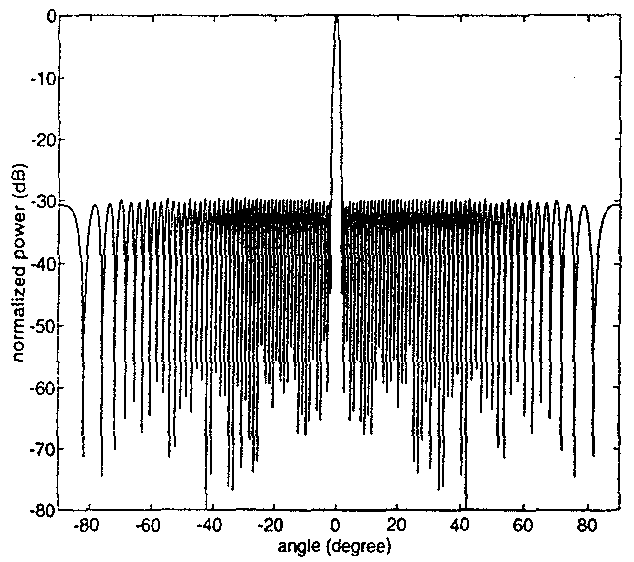
\includegraphics[width=0.8\textwidth,height=0.25\textheight,keepaspectratio]{lms-101-dolph}
    \caption{ДН эталонной решётки из 101 элемента, синтезированной методом Дольфа-Чебышёва}%
    \label{fig:lms-101-dolph}
\end{figure}

\begin{figure}[H]
    \centering
    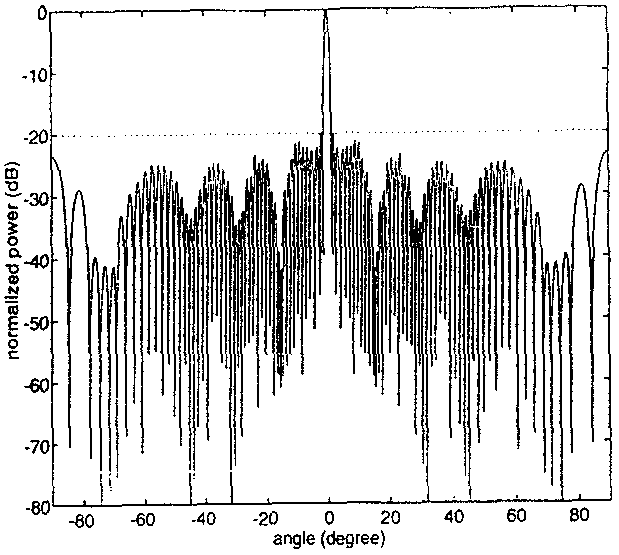
\includegraphics[width=0.8\textwidth,height=0.25\textheight,keepaspectratio]{lms-51-rp}
    \caption{Диаграмма направленности АР из 51 антенного элемента, оптимизированной LMS алгоритмом}%
    \label{fig:lms-51-rp}
\end{figure}

\begin{figure}[H]
    \centering
    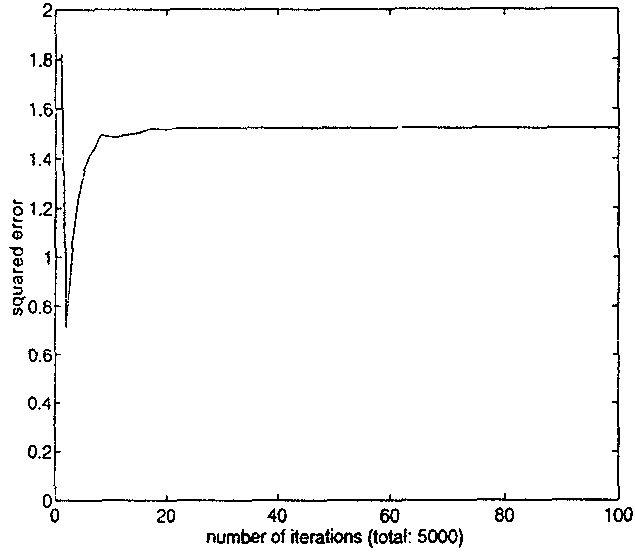
\includegraphics[width=0.8\textwidth,height=0.25\textheight,keepaspectratio]{lms-51-learning-curve}
    \caption{ Кривая обучения LMS алгоритма}%
    \label{fig:lms-51-learning-curve}
\end{figure}




\subsubsection{Вероятностные методы}\label{sec:stochastic-algorithms}

Предыдущие подразделы описывали различные методы нахождения оптимальных распределений с использованием математических 
методов и функций оптимизации. Методы, описанные в данном подразделе, используют различные эволюционные алгоритмы 
для нахождения оптимальных распределений.

Проблема нахождения оптимальных распределений часто рассматривается как комбинаторная задача. Однако с увеличением 
размеров антенных решёток, количество вычислений растёт экспоненциально. \cite{jain2012solving}. Так как вычислительные методы 
с трудом применимы для разреживания больших антенных решёток, на помощь приходят вероятностные методы. Данная группа 
методов включает в себя генетические алгоритмы, муравьиные (ant colony algorithm) и 
кошачьи (cat swarm optimization) алгоритмы, метод роя частиц (particle swarm optimization), 
алгоритм классной комнаты (Teaching-learning-based optimization) и другие. 

Задача оптимизации антенной решётки с точки зрения комбинаторики является дискретной, комбинаторной и NP полной, что 
означает, что время расчёта значительно возрастает при использовании классических методов. В то же время стохастические 
методы позволяют более эффективно решать проблемы приближенного поиска глобального максимума или минимума во 
всё возрастающем пространстве решений. 

В качестве примера рассмотрим алгоритмы, описанные в \cite{jain2012solving} и \cite{luo2015synthesis}. 

Основы эволюционных алгоритмов следующие:
\begin{itemize}
    \item Популяция в генетических алгоритмах состоит из множества решений, представленных уникальными “хромосомами”. 
    Хромосома -- это закодированная строка, в которой каждый символ представляет один параметр решения
    \item Каждый индивидуум (каждое решение) оценивается на основе некоторой функции пригодности, которая сравнивает 
    полученное решение с другими и с эталонными
    \item На основе результатов функции селекции (пригодности) выбираются решения для создания следующего поколения через 
    генетические операции, такие как мутация и кроссовер. Кроссовер -- генетический оператор, который создаёт потомство как 
    комбинацию параметров двух родителей. Мутация -- случайное изменение в параметрах отдельных хромосом. Мутация нужна для 
    избежания локальных экстремумов и поддержания генетического разнообразия в пространстве решений.
\end{itemize}

В работах \cite{jain2012solving} и \cite{luo2015synthesis} генетические алгоритмы применяются следующим образом:

\begin{itemize}
    \item Алгоритм применяется к изначально созданному равномерному распределению на плоском раскрыве. Рассматриваются 
    прямоугольная и круглая решётки соответветственно. 
    \item На каждом шаге алгоритм отключает и включает отдельные элементы решётки
    \item У каждого элемента всего 2 состояния, таким образом каждый ген хромосомы кодируется одним битом и может
    принимать значения либо 0 либо 1.
\end{itemize}


\begin{figure}[H]
    \centering
    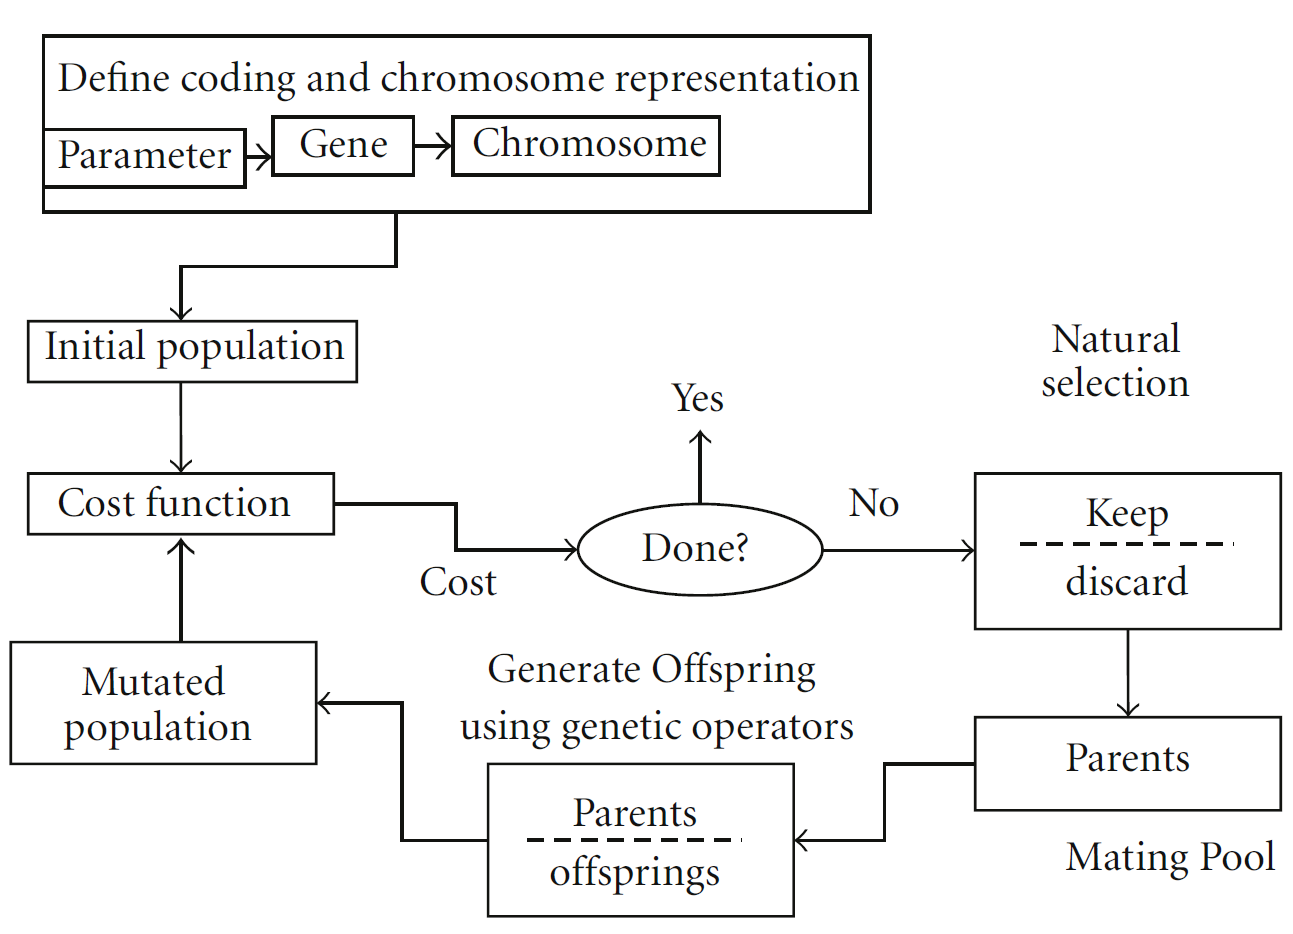
\includegraphics[width=0.8\textwidth,height=0.3\textheight,keepaspectratio]{genetic-algorithm-explanation}
    \caption{Блок-схема простейшего генетического алгоритма}%
    \label{fig:genetic-algorithm-explanation}
\end{figure}

На Рисунках~\ref{fig:genetic-algorithm-pattern-3060}-\ref{fig:genetic-algorithm-pattern-6000} показаны результаты работы ГА для разных направлений прихода сигнала.

\begin{figure}[H]
    \centering
    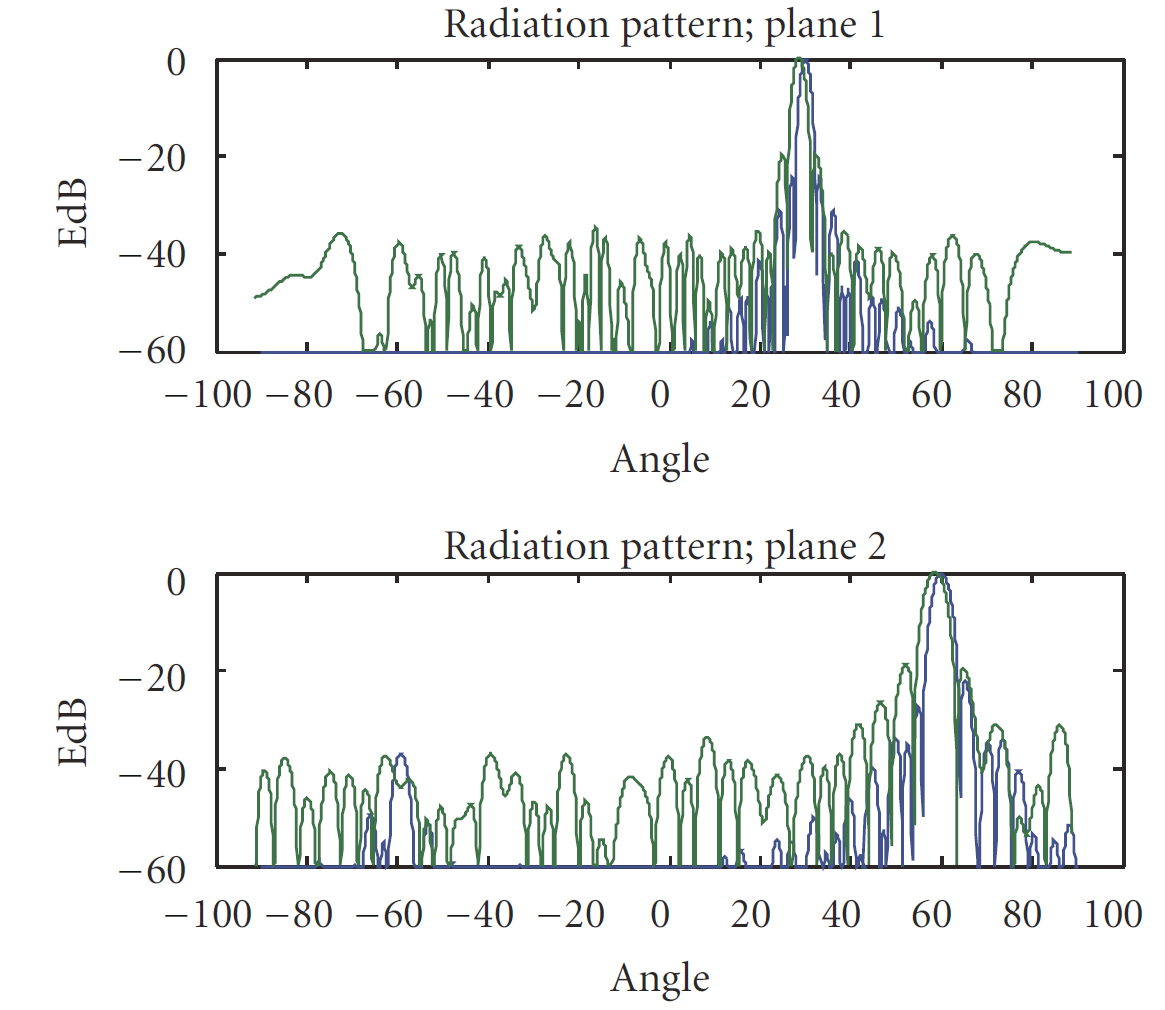
\includegraphics[width=0.8\textwidth,height=0.35\textheight,keepaspectratio]{genetic-algorithm-pattern-3060}
    \caption{ДНА полученной АР в направлении $\theta=30$, $\phi=60$}%
    \label{fig:genetic-algorithm-pattern-3060}
\end{figure}


\begin{figure}[H]
    \centering
    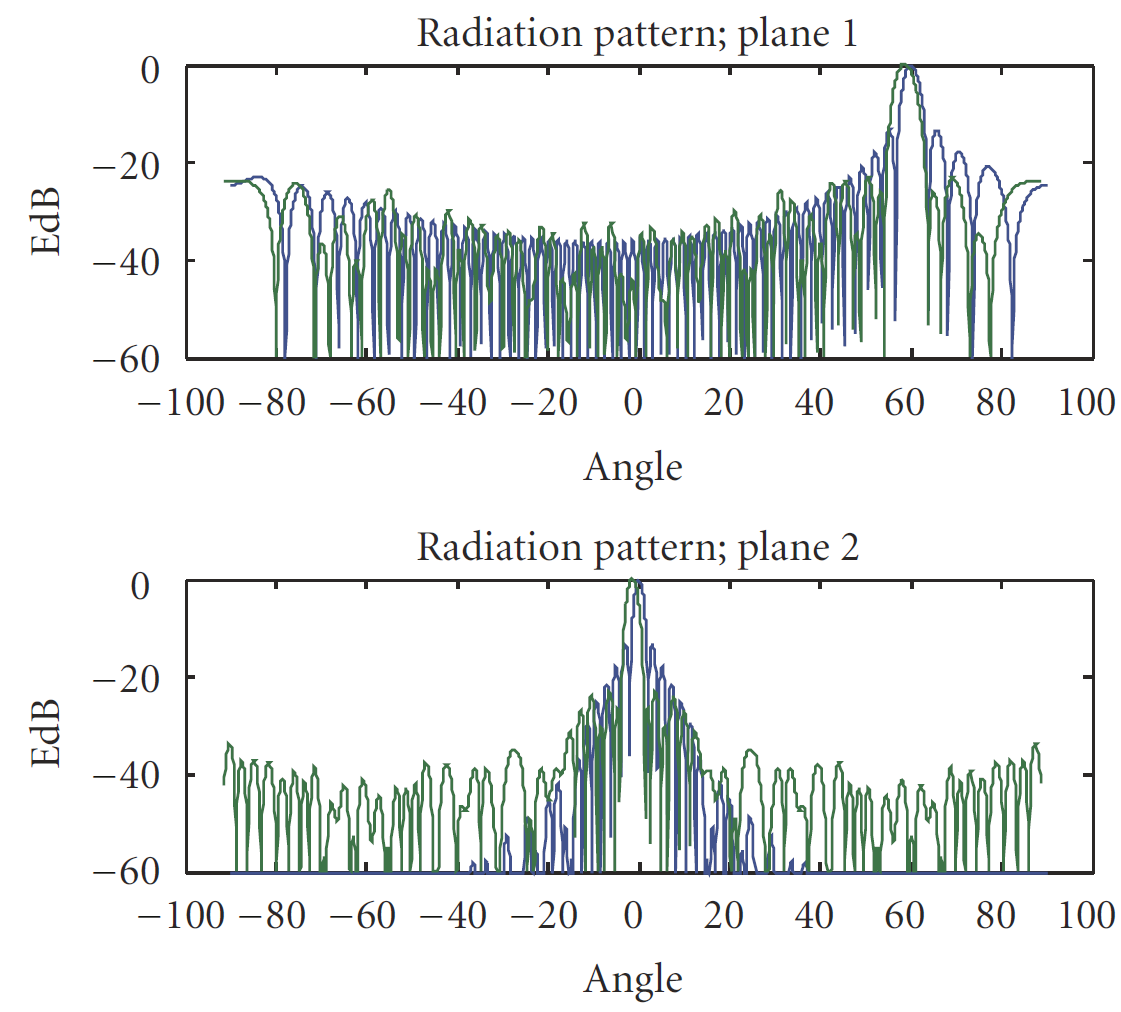
\includegraphics[width=0.8\textwidth,height=0.35\textheight,keepaspectratio]{genetic-algorithm-pattern-6000}
    \caption{ДНА полученной АР в направлении $\theta=60$, $\phi=0$}%
    \label{fig:genetic-algorithm-pattern-6000}
\end{figure}

\subsection{Цифровые антенные решётки}\label{sect:daa}

Цифровые антенные решётки (ЦАР) представляют собой передовую технологию в области антенных систем. ЦАР позволяют 
управлять антенной на цифровом уровне, что обеспечивает большую гибкость гибкость и точность формирования ДН, а также 
синтеза многолучевых систем.

Цифровые антенные решётки основаны на тех же принципах что и классические АФАР, однако отличаются по своей архитектуре. 
Каждый канал в ЦАР представляет собой отдельный цифровой радиоприёмник. Принятые данные обрабатываются в цифровой 
подсистеме на ПЛИС и высокопроизводительных процессорах. 

Преимущества цифровых антенных решёток:

\begin{enumerate}
    \item Большая гибкость в формировании диаграммы направленности
    \item Эффективное формирование многолучевых ДН. Так как вся обработка происходит в цифровом виде, 
    то можно формировать сложные сигналы без потерь на сумматорах/делителях мощности. Особенно в приёмных ЦАР
    \item Увеличение скорости сканирования - различные алгоритмы цифровой обработки сигналов 
    (например алгоритм быстрого преобразования Фурье) позволяют значительно ускорить построение 
    картины сканирования пространства
\end{enumerate}

Проблемы и недостатки ЦАР:

\begin{enumerate}
    \item Сложность разработки - ЦАР представляют собой более сложные, многоканальные радиотехнические устройства 
    со своими особенностями.
    \item Повышенные требования к теплоотводу - высокая интеграция цифровых и аналоговых микросхем повышает 
    требования к теплоотводу, так как на меньшей площади теперь выделяется больше энергии.
    \item Увеличение сложности оборудования обработки данных - ЦАР генерирует большой поток данных, 
    который необходимо успевать обрабатывать
\end{enumerate}

Следующие разделы описывают методы оптимизации с использованием цифровых антенных решёток.
\subsection{Итеративный метод диаграммообразования}\label{sect:iterative-theory}

\subsubsection{Обзор существующих решений}

Идея поиска положения цели в систем радиолокации и радионавигации за счёт использования нескольких систем не нова. 
Так, например, радиосистемы посадки самолётов сантиметрового диапазона применяют два радиолокатора - азимутальный 
и угломестный. Каждый из этих радиолокаторов имеет узкую диаграмму направленности лишь в одной плоскости, и широкую в 
другой. Такой подход позволяет ускорить поиск цели. Местонахождение искомого летательного аппарата определяется в 
полярных координатах на пересечении этих ДН \cite{BakulevSosnovsky2005}.

\begin{figure}[H]
    \centering
    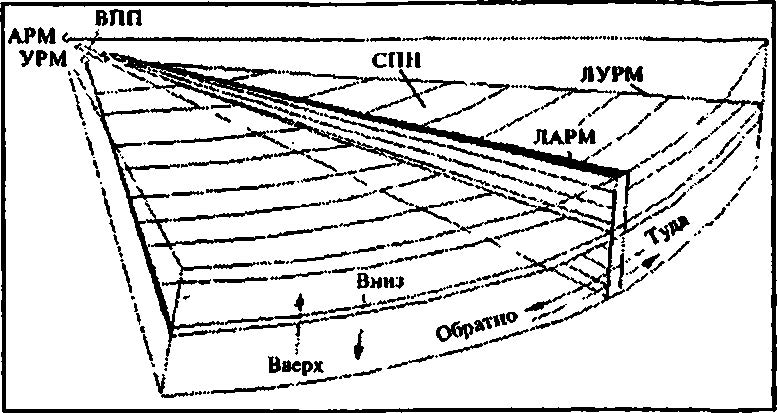
\includegraphics[width=0.8\textwidth,height=0.35\textheight,keepaspectratio]{cm-wave-plane-landing-system}
    \caption{Сектор пропорционального наведения АРМ и УРМ \cite{BakulevSosnovsky2005}}%
    \label{fig:cm-wave-plane-landing-system}
\end{figure}

Похожий подход применяют фазовые дальномерные РНС такие как РНС “Omega”. Для оценки нескольких областей поиска 
применяются сигналы на разных частотах - низкочастотный проводят грубую оценку и позволяют устранить 
неопределённость/многовариативность местоположения объекта, а высокочастотные уточняют местоположение внутри 
выбранной области \cite{BakulevSosnovsky2005}.

\begin{figure}[H]
    \centering
    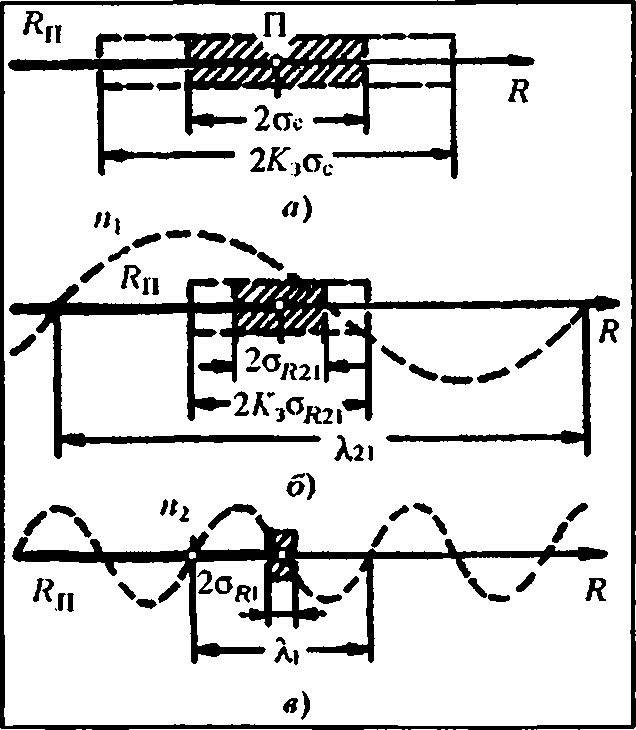
\includegraphics[width=0.8\textwidth,height=0.35\textheight,keepaspectratio]{phase-distance-measurment}
    \caption{Поиск местоположения на (а) грубой (б) средней и (в) точной шкалах \cite{BakulevSosnovsky2005}}%
    \label{fig:phase-distance-measurment}
\end{figure}

Более похожий на предлагаемый подход применяется в РЛС таких как “Воронеж” и “Небо-СВ”. В состав этих систем входит 
несколько АР разных диапазонов. Антенные решётки метрового диапазона проводят грубую оценку на больших дистанциях, 
а АР сантиметрового диапазона осуществляют точную оценку параметров цели и слежение.

\subsubsection{Описание метода}

Рассматриваемый метод предлагает использовать одни и те же данные по несколько раз в разных комбинациях для 
формирования итоговой ДН.

На Рисунке \ref{fig:iterative-method-element-placing} показано расположение элементов в антенной решётке. Также для сравнения 
приведена эквидистантная решётка таких же размеров. Рассматриваемая решётка получена из эквидистантной путём 
удаления элементов на краях антенны. 

\begin{figure}[!ht]
    \centering
    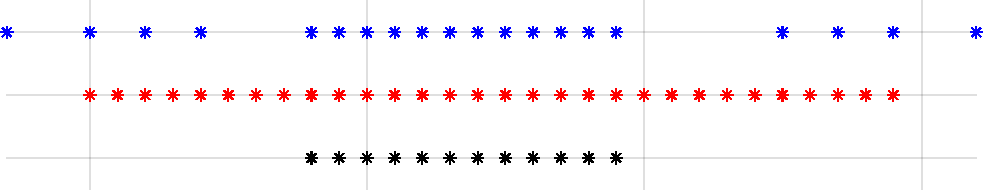
\includegraphics[width=0.8\textwidth,height=0.35\textheight,keepaspectratio]{iterative-method-element-placing}
    \caption{Расположение элементов в эквидистантной решётке (красный), рассматриваемой решётке (синий) и эквидистантной подрешётке (чёрный)}%
    \label{fig:iterative-method-element-placing}
\end{figure}

Формирование ДН данным методом разделено на следующие шаги:

\begin{enumerate}
    \item Проектирование разреженной антенной решётки
    
    За основу берётся модель эквидистантной антенной решётки, из которой удаляются элементы таким образом, что чем ближе к 
    краю будут расположены элементы, тем больше будет расстояние до следующего элемента. Затем к краям добавляются 
    два элемента, расстояние до них определяется тем же принципом.
    \item Принятый сигнал получается за счёт применения формирующих коэффициентов к двум решёткам - полной, т.е. ко 
    всем элементам разреженной решётки; краевым подрешёткам, т.е. ко всем кроме составляющих центральную подрешётку; 
    и к центральной подрешётке
    \item После того как сигналы в каналах будут умножены на соответствующие коэффициенты, проводится 
    свёртка полученных результатов и последующее сканирование
\end{enumerate}

В разделе \ref{sect:iterative-modeling} проведено моделирование данного метода, приведены достоинства, недостатки и возможные пути развития.
\subsection{Применение интерполяции для улучшения характеристик ДН}\label{sect:interpolation-theory}

Рассмотрим приём сигнала с некоторого направления с помощью антенной решётки. 
Модель АР показана на Рисунке \ref{fig:antenna-array-interference}.

\begin{figure}[!ht]
    \centering
    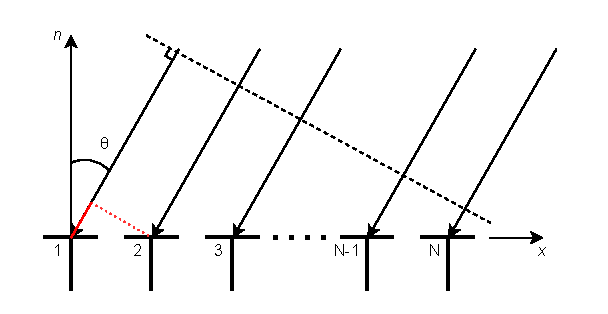
\includegraphics[width=0.8\textwidth,height=0.35\textheight,keepaspectratio]{antenna-array-interference}
    \caption{Приём сигнала на системе антенных элементов}%
    \label{fig:antenna-array-interference}
\end{figure}

Волновой фронт приходящего сигнала примем за плоский, т.к. цель находится в дальней зоне \cite{Chist2012}. 
Амплитуда напряжённости поля одинакова для всех элементов, однако фаза изменяется линейно в 
соответствии с направлением прихода сигналов. 
Примем расстояние от волнового фронта до 0-го элемента решётки за 0. 
Тогда для остальных элементов расстояние до фазового фронта может быть вычислено по формуле

\begin{equation*}
    d_n=x_n \cdot \sin\theta
\end{equation*}

\noindent здесь $x_n$ -- координата элемента в системе отсчёта с $0$ в начале антенной решётки и осью $Ox$ проведённой вдоль 
плоскости АР. $\theta$ -- угол между направлением прихода сигнала и нормалью к плоскости антенной решётки. 

Отсюда набег фазы для n-го элемента можно записать как 

\begin{equation*}
    \phi_n = k x_n \cdot \sin\theta
\end{equation*}

где $k=\frac{2\pi}{\lambda}=\frac{2\pi f}{c}$ -- волновое число. Здесь $\lambda$ -- длина волны, $f$ -- частота сигнала, $c$ -- скорость света.

Тогда сигнал, наведённый на n-ый элемент рассчитывается по формуле

\begin{equation}\label{eqn:antenna-array-element-value}
    E_n=A\cdot e^{j\cdot 2 \pi f x_n \frac{\sin{(\theta)}}{c}}
\end{equation}

Если объединить значения наведённого сигнала со всех элементов в одну последовательность, 
то получится сигнал комплексной синусоиды.

Период этого сигнала изменяется в зависимости от угла прихода, принимая значения от $0$ до $2\pi fx_n/с$.
Форма сигнала, принятого решёткой, зависит от количества целей. Данный сигнал является суммой частотно ограниченного множества сигналов. 

Зная природу сигнала и правильно выбрав точки для его измерения, можно уменьшить число измерений, 
дополнив снятый сигнал с помощью интерполяции.

В разделе \ref{sect:interpolation-modeling} проведено моделирование данного метода, 
описаны сложности разработки и исследования данного метода, приведены предполагаемые достоинства, 
недостатки и возможные пути развития.


\subsection{MIMO радиолокация}\label{sect:mimo-theory}

Рассмотрим структуру классической антенной решётки, показанную на Рисунке~\ref{fig:antenna-array-interference}. 

Сигнал образованный в каждом направлении пространства (либо полученный с него) является суммой 
излучений/принятых сигналов с каждого антенного элемента.

\begin{equation*}
    E=\sum_{1}^{N} E_n
\end{equation*}

\noindent где $E_n$ находится по уравнению~(\ref{eqn:antenna-array-element-value}).

Диаграммообразование в классических антенных решёток выполняется за счёт синфазного сложения сигналов с разных каналов. 
Установка соответствующего комплексного коэффициента передачи для каждого канала формирует соответствующий волновой фронт 
(угол наклона относительно плоскости антенной решетки) в дальней зоне излучения антенны (либо, соответственно, принимает его). 

Говоря о радиолокации, можно утверждать, что приёмник (как цифровой так и аналоговый), получают информацию о цели из 
фаз сигнала, наведённого на приёмные антенны. Аналогично передающая решётка формирует наибольшее усиление в 
определённом направлении за счёт установки соответствующих фаз в каналах. 

Таким образом, приёмная решётка изменяет коэффициенты в каналах так, чтобы сигнал от цели, который приходит на элементы 
с разной фазой, стал синфазным, а передающая - таким образом, чтобы сигналы от разных каналов 
были приняты на цели с одинаковой фазой. 

Если же передающая решётка будет излучать синфазный сигнал со всех каналов, то у цели они будут приняты, 
и отражены с разной фазой. Если каким-то образом отметить и разделить сигналы от разных каналов передающей решётки, 
то на приёмной можно будет установить направление на цель относительно передающей решётки. 

Общая идея MIMO радиолокаторов заключается в том, что как передающая, так и приёмная решётка являются цифровыми.
Таким образом MIMO радиолокатор представлен множеством антенн, 
которые передают и принимают сигнал независимо друг от друга. 
Затем принятые сигналы проходят совместную обработку для построения множества диаграмм направленности.

\begin{figure}[H]
    \centering
    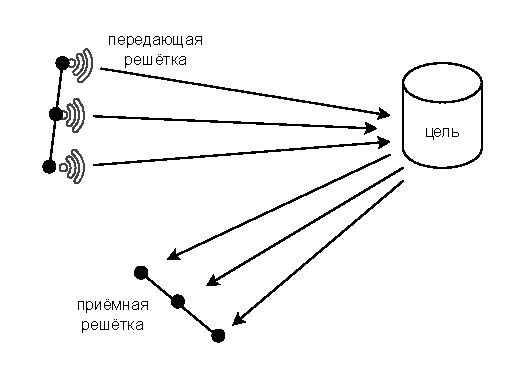
\includegraphics[width=0.8\textwidth,height=0.35\textheight,keepaspectratio]{MIMO-Demo}
    \caption{Иллюстрация MIMO радиолокатора. Положения как приёмных и передающих каналов известны в общем центре обработки данных}%
    \label{fig:mimo-demo}
\end{figure}

В разделе \ref{sect:mimo-modeling} проведено моделирование когерентного MIMO радиолокатора. 
Приведены достоинства и недостатки таких радаров. Описаны перспективы дальнейшего развития.


%
\section{Моделирование классических антенных решёток}\label{sect:distributions-modeling}

\subsection{Описание программы моделирования и визуализации результатов}\label{sect:distributions-modeling-program}

Моделирование различных антенных решёток проводилось в программном пакете Mathworks MATLAB. Диаграмма, описывающая 
работу написанной программы показана на Рисунке~\ref{fig:array-modeling-program-sch}, 
код программы можно увидеть в Приложении~\ref{appendix:arrays-code-appendix}

\begin{figure}[!ht]
    \centering
    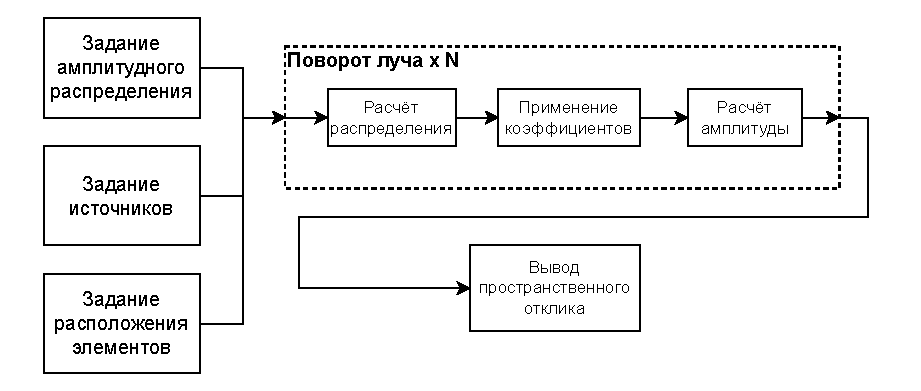
\includegraphics[width=0.8\textwidth,height=0.35\textheight,keepaspectratio]{array-modeling-program-sch}
    \caption{Диаграмма работы программы расчёта}%
    \label{fig:array-modeling-program-sch}
\end{figure}

Процесс работы программы следующий:

\begin{enumerate}
    \item Пользователь вводит амплитуды и направления прихода сигналов
    \item Программа \textit{distribution\_former.m} рассчитывает комплексное распределение на элементах антенны
    \item Промежуточная программа применяет к имеющемуся распределению различные коэффициенты 
    \item Программа \textit{aec\_simulation.m} строит диаграмму направленности и выводит её на экран
\end{enumerate}

В следующих разделах приведены результаты симуляции для антенных решёток, составленных из 24 элементов.

\subsection{Эквидистантная антенная решётка с равномерным распределением амплитуд}

Расположение элементов показано на Рисунке~\ref{fig:equally-spaced-distribution-pos-modeling}. Результаты моделирования отображены на Рисунке~\ref{fig:equally-spaced-distribution-modeling}.

\begin{figure}[!ht]
    \centering
    
\includegraphics[width=0.8\textwidth]{equally-spaced-distribution}
    \caption{Расположение элементов в эквидистантной АР}
    \label{fig:equally-spaced-distribution-pos-modeling}
\end{figure}



\begin{figure}[!ht]
    \centering
    \begin{subfigure}[b]{0.49\textwidth}
        \centering
        \hspace*{-3ex}
        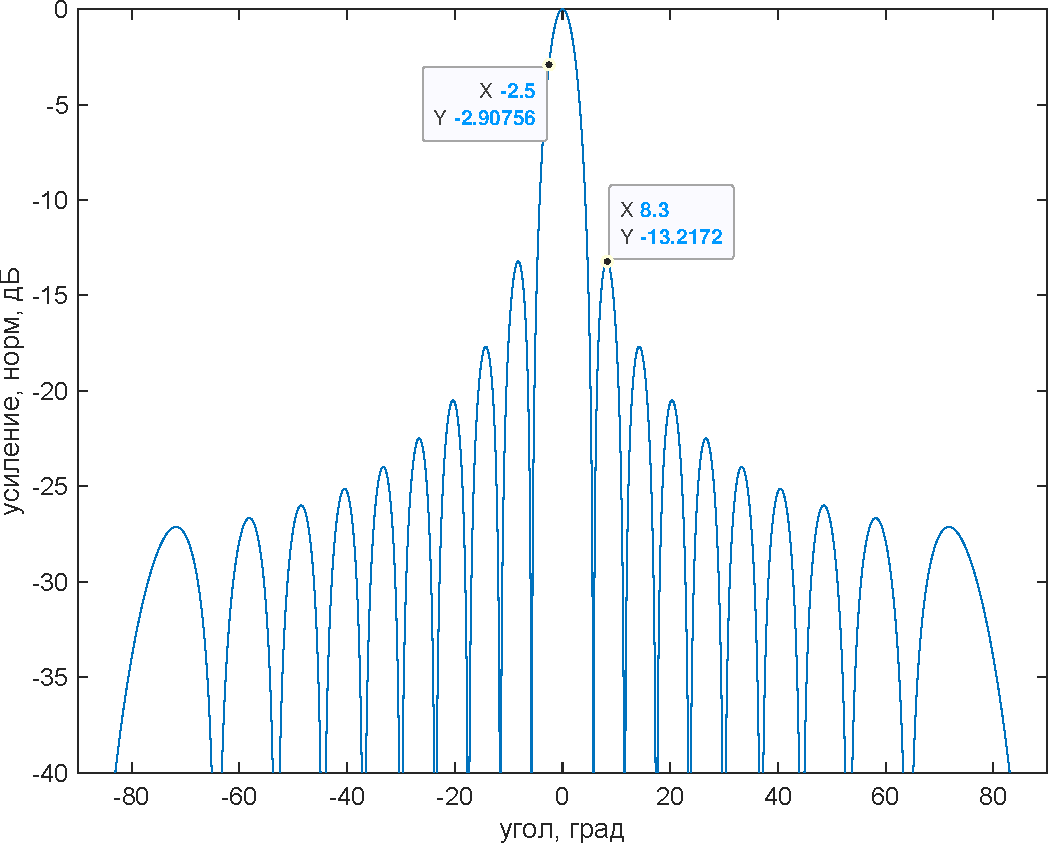
\includegraphics[width=\textwidth]{equally-spaced-distribution-beam-pattern0}
        \caption{}%
    \end{subfigure}
    \hfill
    \begin{subfigure}[b]{0.49\textwidth}
        \centering
        \hspace*{-3ex}
        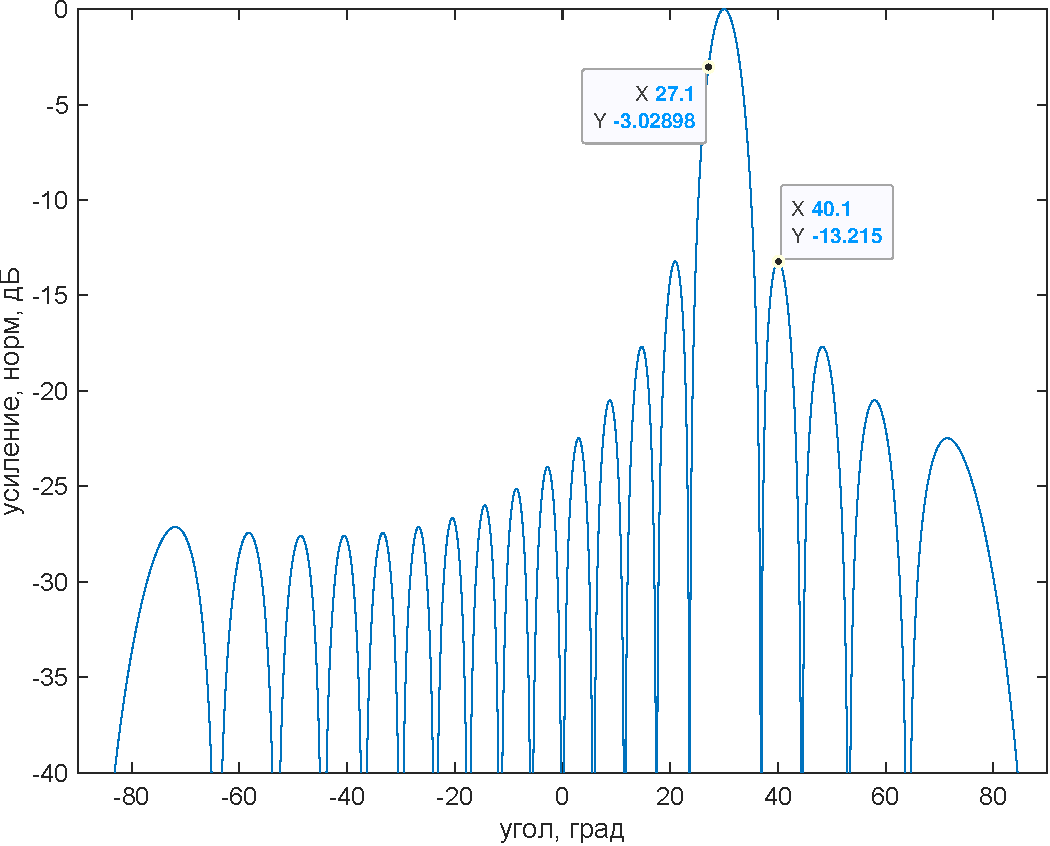
\includegraphics[width=\textwidth]{equally-spaced-distribution-beam-pattern30}
        \caption{}%
    \end{subfigure}
    \caption{%
    Диаграмма направленности АР при направлении главного лепестка на (а) 0 градусов и (б) 30 градусов
    }%
    \label{fig:equally-spaced-distribution-modeling}
\end{figure}

Расстояние между элементами $d=\lambda/2$. Видно, что уровень боковых лепестков составляет $\sim-13$~дБ, 
а ширина главного лепестка равна 5~градусам.

% % %
\subsection{Равномерно спадающее к краям амплитудное распределение}

Расположение элементов показано на Рисунке~\ref{fig:linear-decreasing-amplitude-array-pos}. Результаты моделирования отображены на Рисунке~\ref{fig:linear-decreasing-amplitude-array-modeling}.

\begin{figure}[!ht]
    \centering
    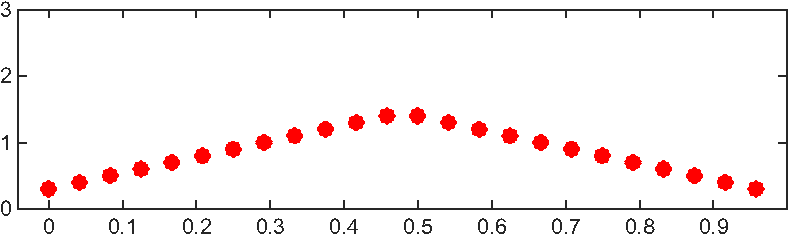
\includegraphics[width=0.8\textwidth]{linear-decreasing-amplitude-array-pos}
    \caption{Расположение элементов в АР}
    \label{fig:linear-decreasing-amplitude-array-pos}
\end{figure}


\begin{figure}[!ht]
    \centering
    \begin{subfigure}[b]{0.49\textwidth}
        \centering
        \hspace*{-3ex}
        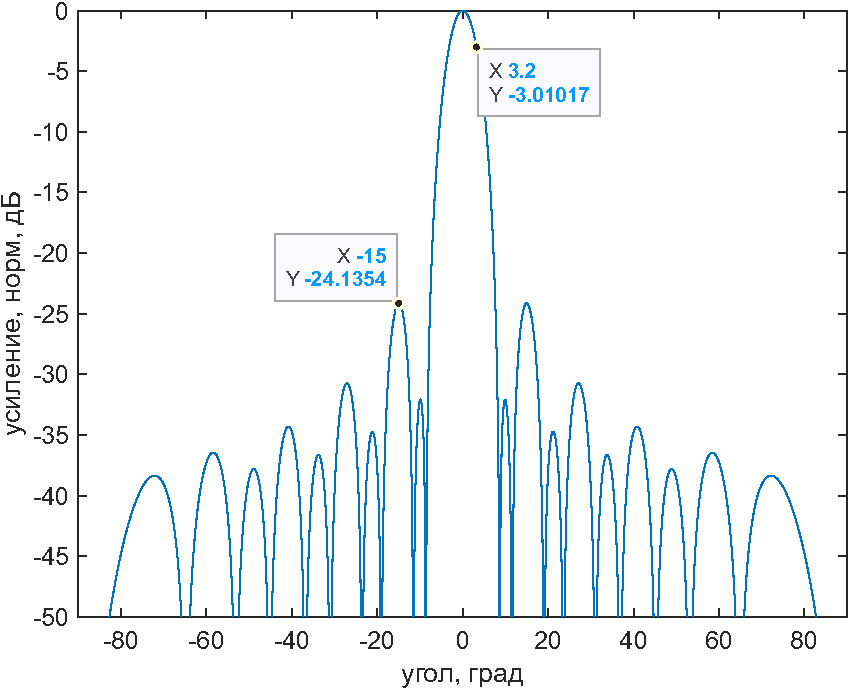
\includegraphics[width=\textwidth]{linear-decreasing-amplitude-array-beam-pattern0}
        \caption{}%
    \end{subfigure}
    \hfill
    \begin{subfigure}[b]{0.49\textwidth}
        \centering
        \hspace*{-3ex}
        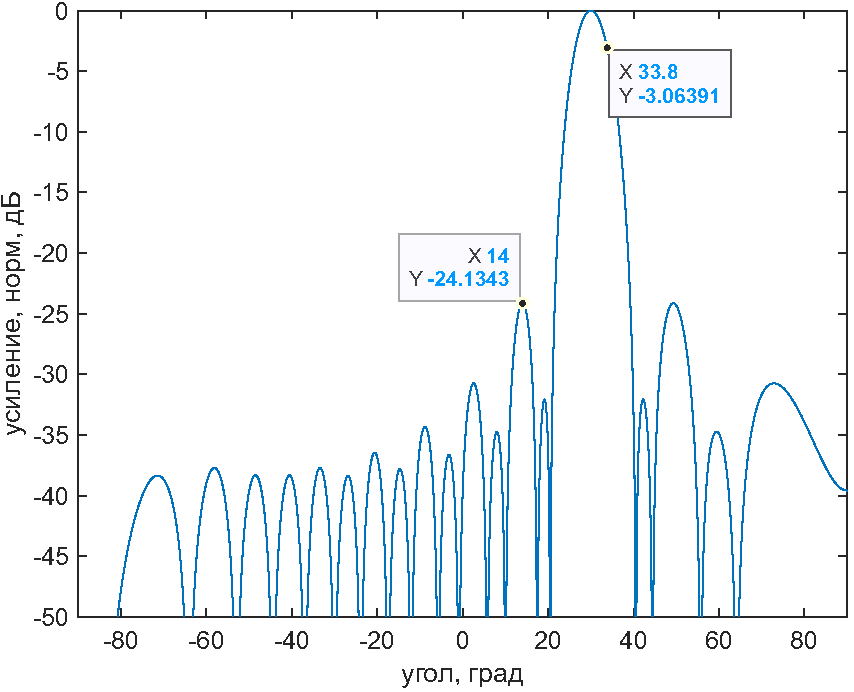
\includegraphics[width=\textwidth]{linear-decreasing-amplitude-array-beam-pattern30}
        \caption{}%
    \end{subfigure}
    \caption{%
    Диаграмма направленности АР при направлении главного лепестка на (а) 0 градусов и (б) 30 градусов
    }%
    \label{fig:linear-decreasing-amplitude-array-modeling}
\end{figure}

Расстояние между элементами $d=\lambda/2$. Видно, что уровень боковых лепестков составляет $\sim-24$~дБ,
что меньше чем при равномерном распределении амплитуд,
а ширина главного лепестка равна $6,2$~градусам, что больше чем при равномерном распределении.

% % %
\subsection{Распределение Дольфа-Чебышева}

Расположение элементов показано на Рисунке~\ref{fig:dolph-tcheby-array-pos}. Результаты моделирования отображены на Рисунке~\ref{fig:dolph-tcheby-array-modeling}.

\begin{figure}[!ht]
    \centering
    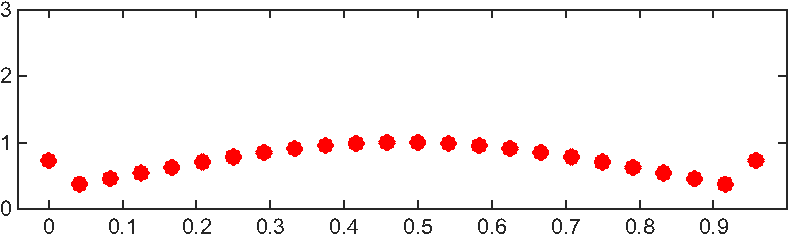
\includegraphics[width=0.8\textwidth]{dolph-tcheby-array-pos}
    \caption{Расположение элементов в АР}
    \label{fig:dolph-tcheby-array-pos}
\end{figure}


\begin{figure}[!ht]
    \centering
    \begin{subfigure}[b]{0.49\textwidth}
        \centering
        \hspace*{-3ex}
        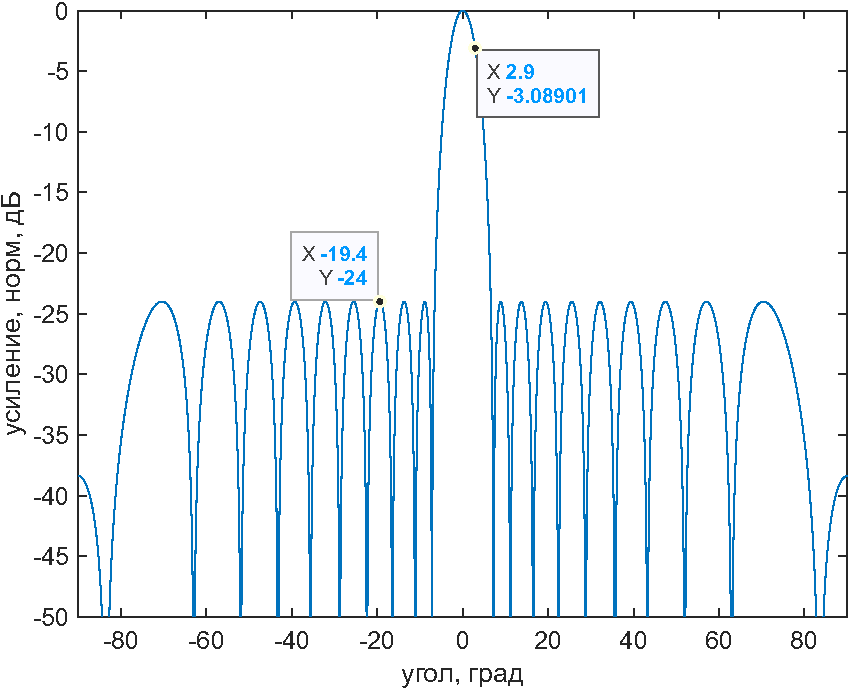
\includegraphics[width=\textwidth]{dolph-tcheby-array-beam-pattern0}
        \caption{}%
    \end{subfigure}
    \hfill
    \begin{subfigure}[b]{0.49\textwidth}
        \centering
        \hspace*{-3ex}
        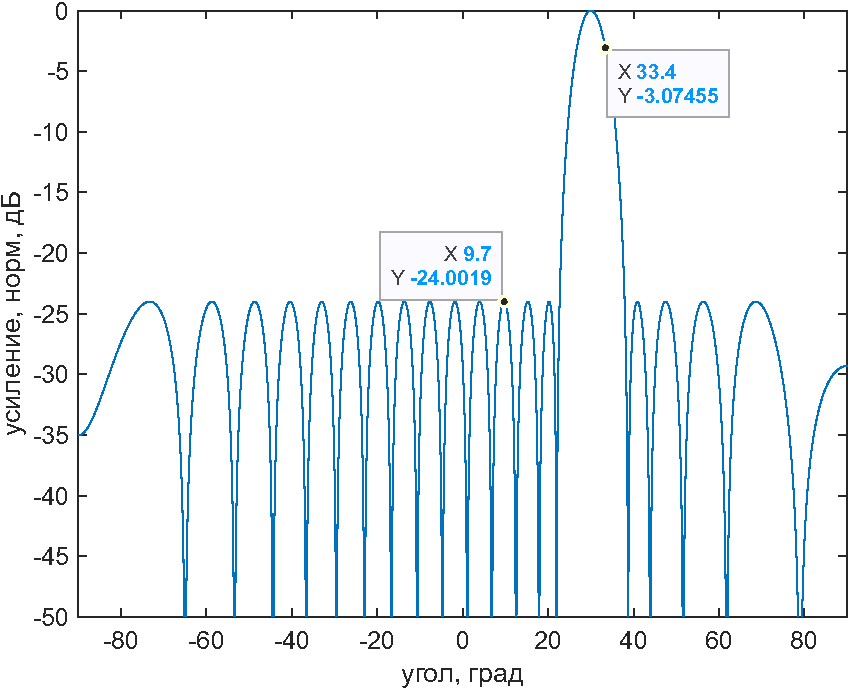
\includegraphics[width=\textwidth]{dolph-tcheby-array-beam-pattern30}
        \caption{}%
    \end{subfigure}
    \caption{%
    Диаграмма направленности АР при направлении главного лепестка на (а) 0 градусов и (б) 30 градусов
    }%
    \label{fig:dolph-tcheby-array-modeling}
\end{figure}

Расстояние между элементами $d=\lambda/2$. Видно, что уровень боковых лепестков составляет $\sim-24$~дБ, 
что меньше чем при равномерном распределении амплитуд, 
а ширина главного лепестка равна $5,8$~градусам, 
что больше чем при равномерном распределении, но меньше чем при равномерно спадающем.

% % %
\subsection{Равномерно возрастающее к краям амплитудное распределение}

Расположение элементов показано на Рисунке~\ref{fig:linear-encreasing-amplitude-array-pos}. Результаты моделирования отображены на Рисунке~\ref{fig:linear-encreasing-amplitude-array-modeling}.

\begin{figure}[!ht]
    \centering
    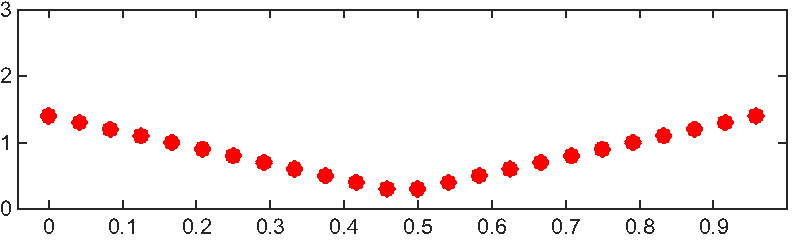
\includegraphics[width=0.8\textwidth]{linear-encreasing-amplitude-array-pos}
    \caption{Расположение элементов в АР}
    \label{fig:linear-encreasing-amplitude-array-pos}
\end{figure}


\begin{figure}[!ht]
    \centering
    \begin{subfigure}[b]{0.49\textwidth}
        \centering
        \hspace*{-3ex}
        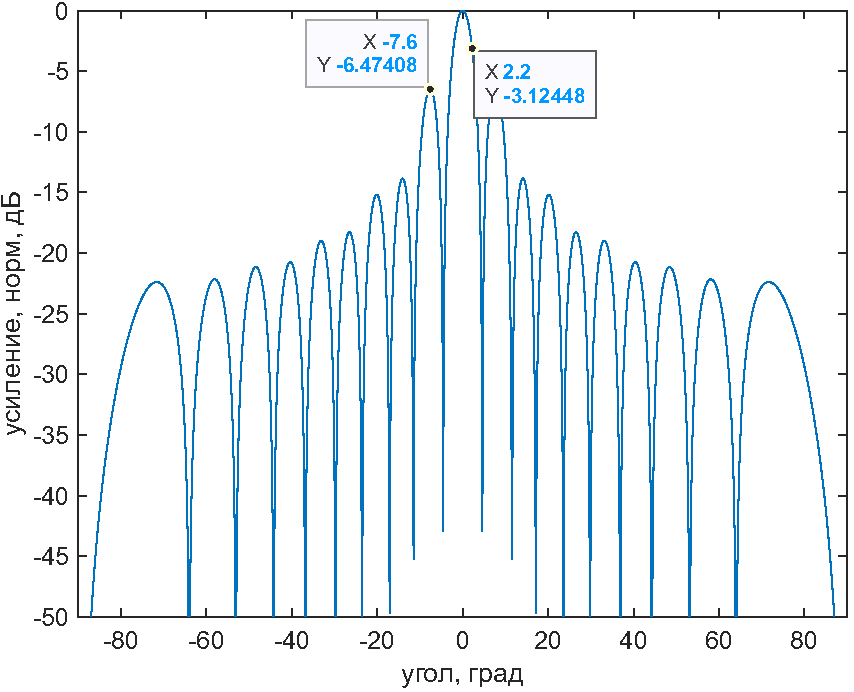
\includegraphics[width=\textwidth]{linear-encreasing-amplitude-array-beam-pattern0}
        \caption{}%
    \end{subfigure}
    \hfill
    \begin{subfigure}[b]{0.49\textwidth}
        \centering
        \hspace*{-3ex}
        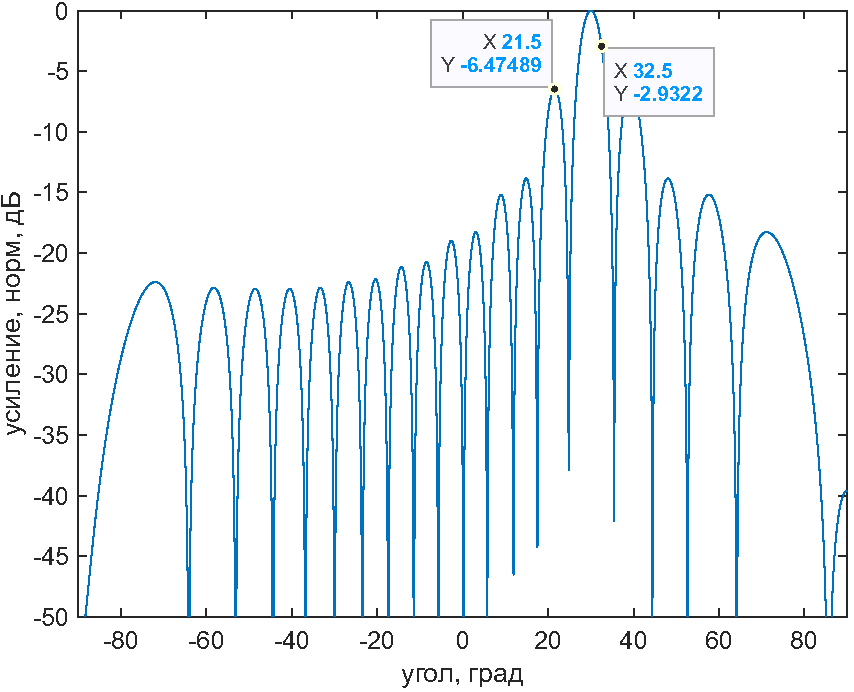
\includegraphics[width=\textwidth]{linear-encreasing-amplitude-array-beam-pattern30}
        \caption{}%
    \end{subfigure}
    \caption{%
    Диаграмма направленности АР при направлении главного лепестка на (а) 0 градусов и (б) 30 градусов
    }%
    \label{fig:linear-encreasing-amplitude-array-modeling}
\end{figure}

Расстояние между элементами $d=\lambda/2$. Видно, что уровень боковых лепестков составляет $\sim-6,4$~дБ, 
что значительно больше чем при равномерном распределении амплитуд, 
однако ширина главного лепестка равна $4,4$~градусам, 
что меньше чем при равномерном распределении.

% % %
\subsection{Расширяющееся к краям геометрическое распределение}

Расположение элементов показано на Рисунке~\ref{fig:side-widing-array-pos}. Результаты моделирования отображены на Рисунке~\ref{fig:side-widing-array-modeling}.

\begin{figure}[!ht]
    \centering
    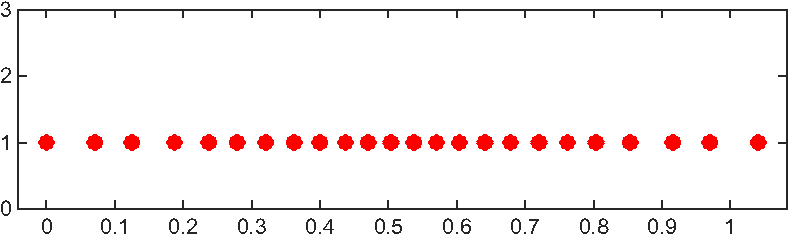
\includegraphics[width=0.8\textwidth]{side-widing-array-pos}
    \caption{Расположение элементов в АР}
    \label{fig:side-widing-array-pos}
\end{figure}


\begin{figure}[!ht]
    \centering
    \begin{subfigure}[b]{0.49\textwidth}
        \centering
        \hspace*{-3ex}
        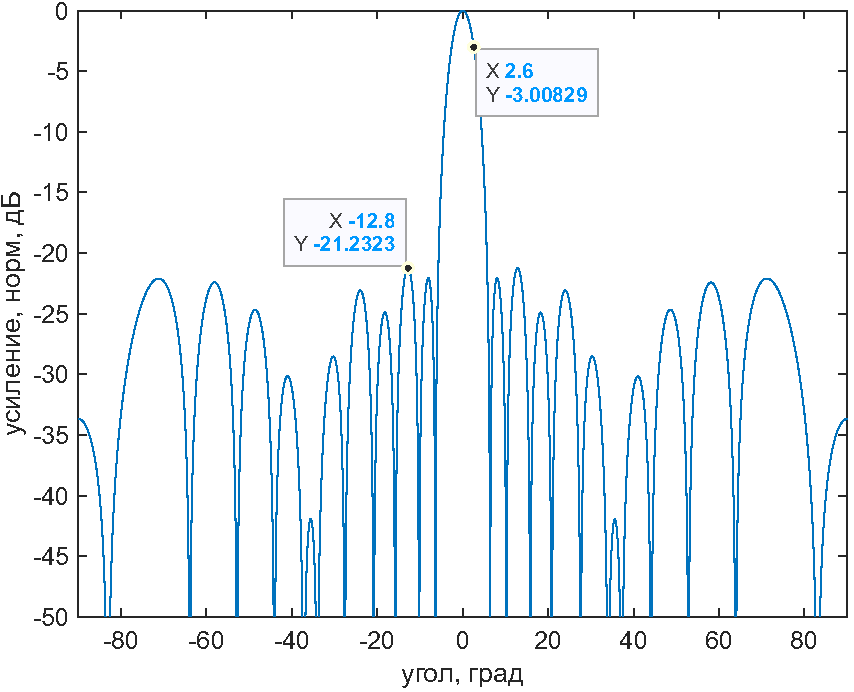
\includegraphics[width=\textwidth]{side-widing-array-beam-pattern0}
        \caption{}%
    \end{subfigure}
    \hfill
    \begin{subfigure}[b]{0.49\textwidth}
        \centering
        \hspace*{-3ex}
        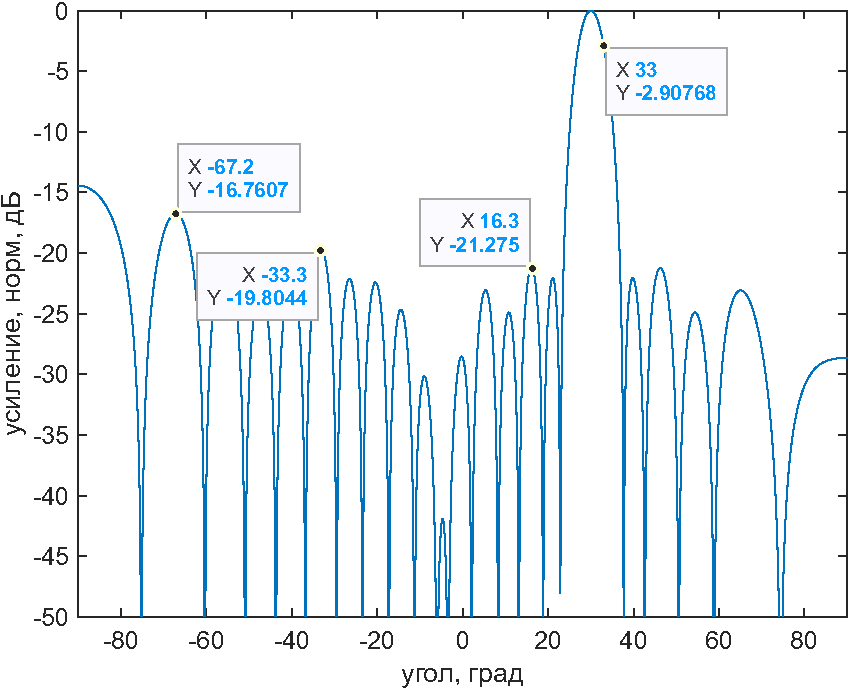
\includegraphics[width=\textwidth]{side-widing-array-beam-pattern30}
        \caption{}%
    \end{subfigure}
    \caption{%
    Диаграмма направленности АР при направлении главного лепестка на (а) 0 градусов и (б) 30 градусов
    }%
    \label{fig:side-widing-array-modeling}
\end{figure}

Расстояние между элементами $d=\lambda/2$. Видно, что уровень боковых лепестков составляет $\sim-21$~дБ, 
что меньше чем в эквидистантной решётке с равномерным распределением амплитуд, 
а ширина главного лепестка равна $5,2$~градусам, 
что немного больше чем при равномерном распределении.

При этом при отклонении на $30$~градусов заметны дифракционные лепестки на уровне $-15$~дБ, в отклонении $-90$ градусов от нормали ($120$~градусов от главного лепестка); а УБЛ составляет $-21 \div -19$~дБ, что также меньше чем при равномерном распределении.

% % %
\subsection{Сужающееся к краям геометрическое распределение}

Расположение элементов показано на Рисунке~\ref{fig:side-narrowing-array-pos}. Результаты моделирования отображены на Рисунке~\ref{fig:side-narrowing-array-modeling}.

\begin{figure}[!ht]
    \centering
    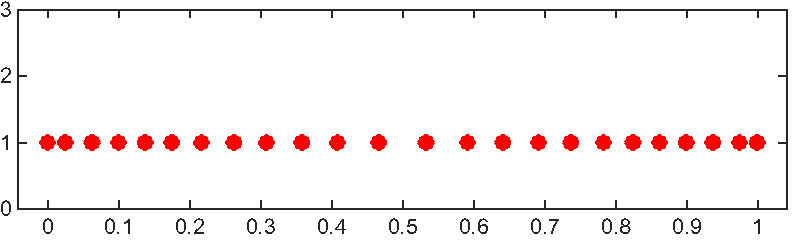
\includegraphics[width=0.8\textwidth]{side-narrowing-array-pos}
    \caption{Расположение элементов в АР}
    \label{fig:side-narrowing-array-pos}
\end{figure}


Расстояние между элементами $d=\lambda/2$. Видно, что уровень боковых лепестков составляет $\sim-10$~дБ, 
что больше чем в эквидистантной решётке с равномерным распределением амплитуд, 
однако ширина главного лепестка равна $4,4$~градусов, 
что меньше чем при равномерном распределении.

\begin{figure}[H]
    \centering
    \begin{subfigure}[b]{0.49\textwidth}
        \centering
        \hspace*{-3ex}
        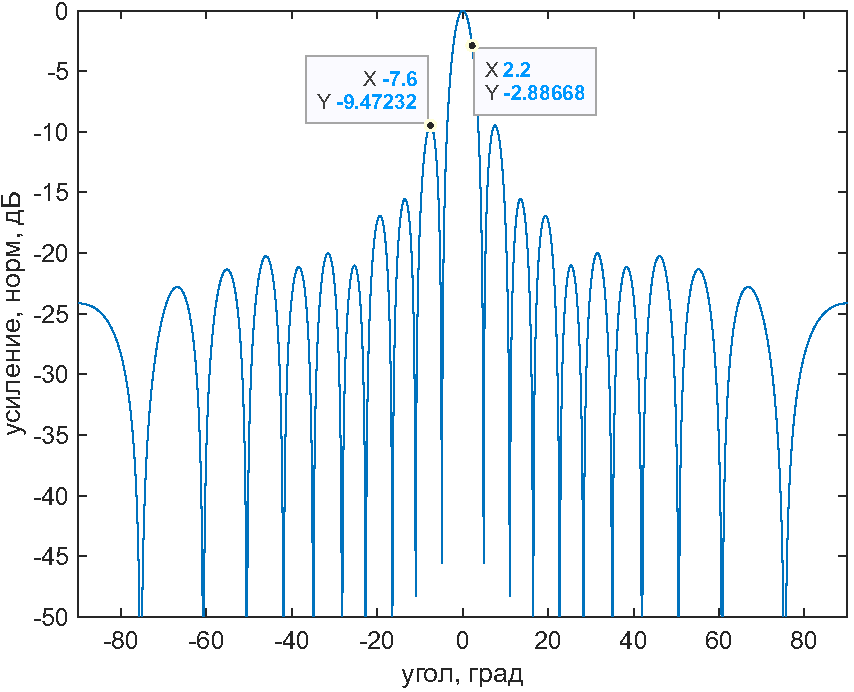
\includegraphics[width=\textwidth]{side-narrowing-array-beam-pattern0}
        \caption{}%
    \end{subfigure}
    \hfill
    \begin{subfigure}[b]{0.49\textwidth}
        \centering
        \hspace*{-3ex}
        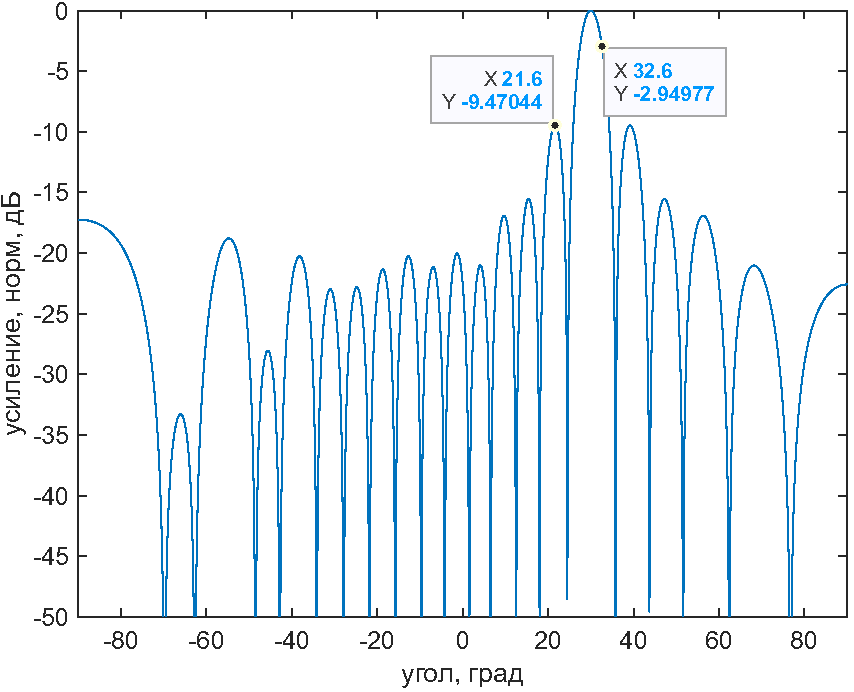
\includegraphics[width=\textwidth]{side-narrowing-array-beam-pattern30}
        \caption{}%
    \end{subfigure}
    \caption{%
    Диаграмма направленности АР при направлении главного лепестка на (а) 0 градусов и (б) 30 градусов
    }%
    \label{fig:side-narrowing-array-modeling}
\end{figure}



% % %
\subsection{Заключение}

По результатам моделирования можно заметить, что концентрация энергии в центре АР уменьшает УБЛ, однако 
увеличивает ширину основного лепестка. В свою очередь уменьшение концентрации энергии в центре АР и увеличение её 
по краям, позволяет немного уменьшить ширину главного лепестка, однако при этом значительно возрастает УБЛ.

Если изменять распределение энергии за счёт изменения положения элементов, то можно получить меньший УБЛ, по 
сравнению с эквидистантными решётками с равным и меньшим количеством элементов, однако при этом будет 
возрастать УДЛ. В то же время можно уменьшать УДЛ по сравнению с эквидистантными решётками, с 
межэлементным расстоянием $d>\lambda/2$, однако при этом, как правило возрастает УБЛ. При этом в обоих случаях, 
ширина главного лепестка остаётся такой же как у эквидистантных решёток либо становится меньше.

Для расчёта распределений в решётках с относительно небольшим количеством элементов удобно применять 
методы, использующие математические приближения, однако для АР с большим числом элементов более выгодным 
становится применение различных генетических алгоритмов либо ручной оптимизации структур с 
изначально нестандартным расположением элементов.

Применение неравномерных распределений позволяет гибко настраивать параметры 
диаграммы направленности антенных решёток. Данный подход имеет следующие преимущества:

\begin{itemize}
    \item Уменьшение УБЛ относительно решёток с равным межэлементным расстоянием
    \item Уменьшение уровня дифракционных лепестков по сравнению с АР с межэлементным расстоянием $d>\lambda/2$
    \item Увеличенная рабочая полоса по сравнению с эквидистантными решётками \cite{andreasen1962linear}
    \item Уменьшение числа элементов по сравнению с 
    эквидистантными решётками со схожими характеристиками направленности
    \item По сравнению с методами, представленными далее, данный подход не требует сложной системы обработки сигнала
\end{itemize}

В то же время данный подход имеет ряд недостатков:

\begin{itemize}
    \item Решётки с неравномерным амплитудным распределением имеют более сложную систему 
    запитки антенных элементов, т.е. более дорогой приемопередающий тракт
    \item Некоторые распределения для неэквидистантных решёток, например вариант 
    из \cite{harrington1961sidelobe}, располагают элементы на расстоянии меньше половины длины волны, 
    из-за чего становится более важно учитывать 
    ЭМ-взаимодействие между элементами \cite{andreasen1962linear}, \cite{ishimaru1962theory}
    \item Разреженные решётки имеют меньший кооэффициент усиления по сравнению с 
    эквидистантными \cite{andreasen1962linear} ввиду меньшего количества антенных элементов
    \item При больших размерах решёток, методы поиска неравномерных геометрических распределений усложняются, 
    а имеющиеся алгоритмы могут давать оптимальные но не наилучшие решения с точки зрения 
    характеристик направленности, хотя и дают выигрыш в стоимости
\end{itemize}
\section{Моделирование диаграммообразования итеративным методом}\label{sect:iterative-modeling}

Программа для моделирования схожа с той, что использовалась 
в разделе с амплитудными и геометрическими распределениями. 
Моделирование проводилось для антенной решётки, заданной согласно методу, описанному в разделе~\ref{sect:iterative-theory}.

Установим координаты исходной эквидистантной решётки

\begin{minted}[
    linenos,
    breaklines,
    frame=single,
    framesep=10pt
]{matlab}
f = 3e9; % 3 GHz text
lam = freq2wavelen(f); % длина волны
xmin = 0;xmax = 29; % количество элементов
dOk = lam/2; % межэлементное расстояние
dxOk = dOk*(xmin:1:xmax)'; % координаты элементов     
\end{minted}

Сформируем исследуемую разреженную решётку с помощью удаления 12 элементов из исходной решётки и 
добавления двух элементов на её краях. Отдельно зададим центральную эквидистантную подрешётку.

\begin{minted}[
    linenos,
    firstnumber=last,
    breaklines,
    frame=single,
    framesep=10pt
]{matlab}
dxRare = [-2*dOk; dxOk([1 3 5 9:20 26 28 30]); 33*dOk];
dxRare2 = dxOk([9:20]);   
\end{minted}

Получим распределения сигналов на заданных решётках

\begin{minted}[
    linenos,
    firstnumber=last,
    breaklines,
    frame=single,
    framesep=10pt
]{matlab}
valuesOk = distribution_former(dxOk,f,aimAngles, aimAmps); % значение сигнала на элементах исходной решётки
valuesRare = distribution_former(dxRare,f,aimAngles, aimAmps);  % значение сигнала на элементах исходной решётки
valuesRare2 = valuesOk([9:20]); % значение сигнала на центральной подрешётке
\end{minted}

Дополнительно формируются значения со спадающими амплитудными распределениями

\begin{minted}[
    linenos,
    firstnumber=last,
    breaklines,
    frame=single,
    framesep=10pt
]{matlab}
valuesRare1 = valuesRare.*([[1,1, 3, 5, 6, 6.5, 7, 7.4, 7.7,8] fliplr([1,1, 3, 5, 6, 6.5, 7, 7.4, 7.7,8])]');
valuesRare21 = valuesRare2.*([[5, 5, 5.5, 6, 6, 6.5] fliplr([5, 5, 5.5, 6, 6, 6.5])]');  
\end{minted}

Далее проводится сканирование и перемножение пространственных откликов

\begin{minted}[
    linenos,
    firstnumber=last,
    breaklines,
    frame=single,
    framesep=10pt
]{matlab}
[rstOk,theta] = aec_simulation(valuesOk, dxOk,f); % ДН эквидистантной решётки для сравнения
rstRare = aec_simulation(valuesRare, dxRare,f); % ДН разрженной решетки для сравнения
rstRare1 = aec_simulation(valuesRare1, dxRare,f);
rstRare2 = aec_simulation(valuesRare2, dxRare2,f); % ДН центарльной решётки для сравнения
rstRare21 = aec_simulation(valuesRare21, dxRare2,f);
rstRare3 = rstRare21.*rstRare; % результирующая ДН
\end{minted}

Для оценки результатов работы данного алгоритма, по методу из раздела~\ref{sec:perturbations-method} был сформирован 
ещё один разреженный массив с расширяющимся к краям геометрическим распределением.

Рассмотрим результаты моделирования на Рисунке~\ref{iterative-array-raw-beam-pattern}. Как видно, отклик разреженных 
решёток имеет сравнимый по ширине главный лепесток, однако ДН решётки разреженной методом 
удаления имеет даже бОльшую величину УБЛ, чем у эквидистантной, 
и при этом обе разреженные решётки имеют довольно высокие уровни дифракционных лепестков.

\begin{figure}[!ht]
    \centering
    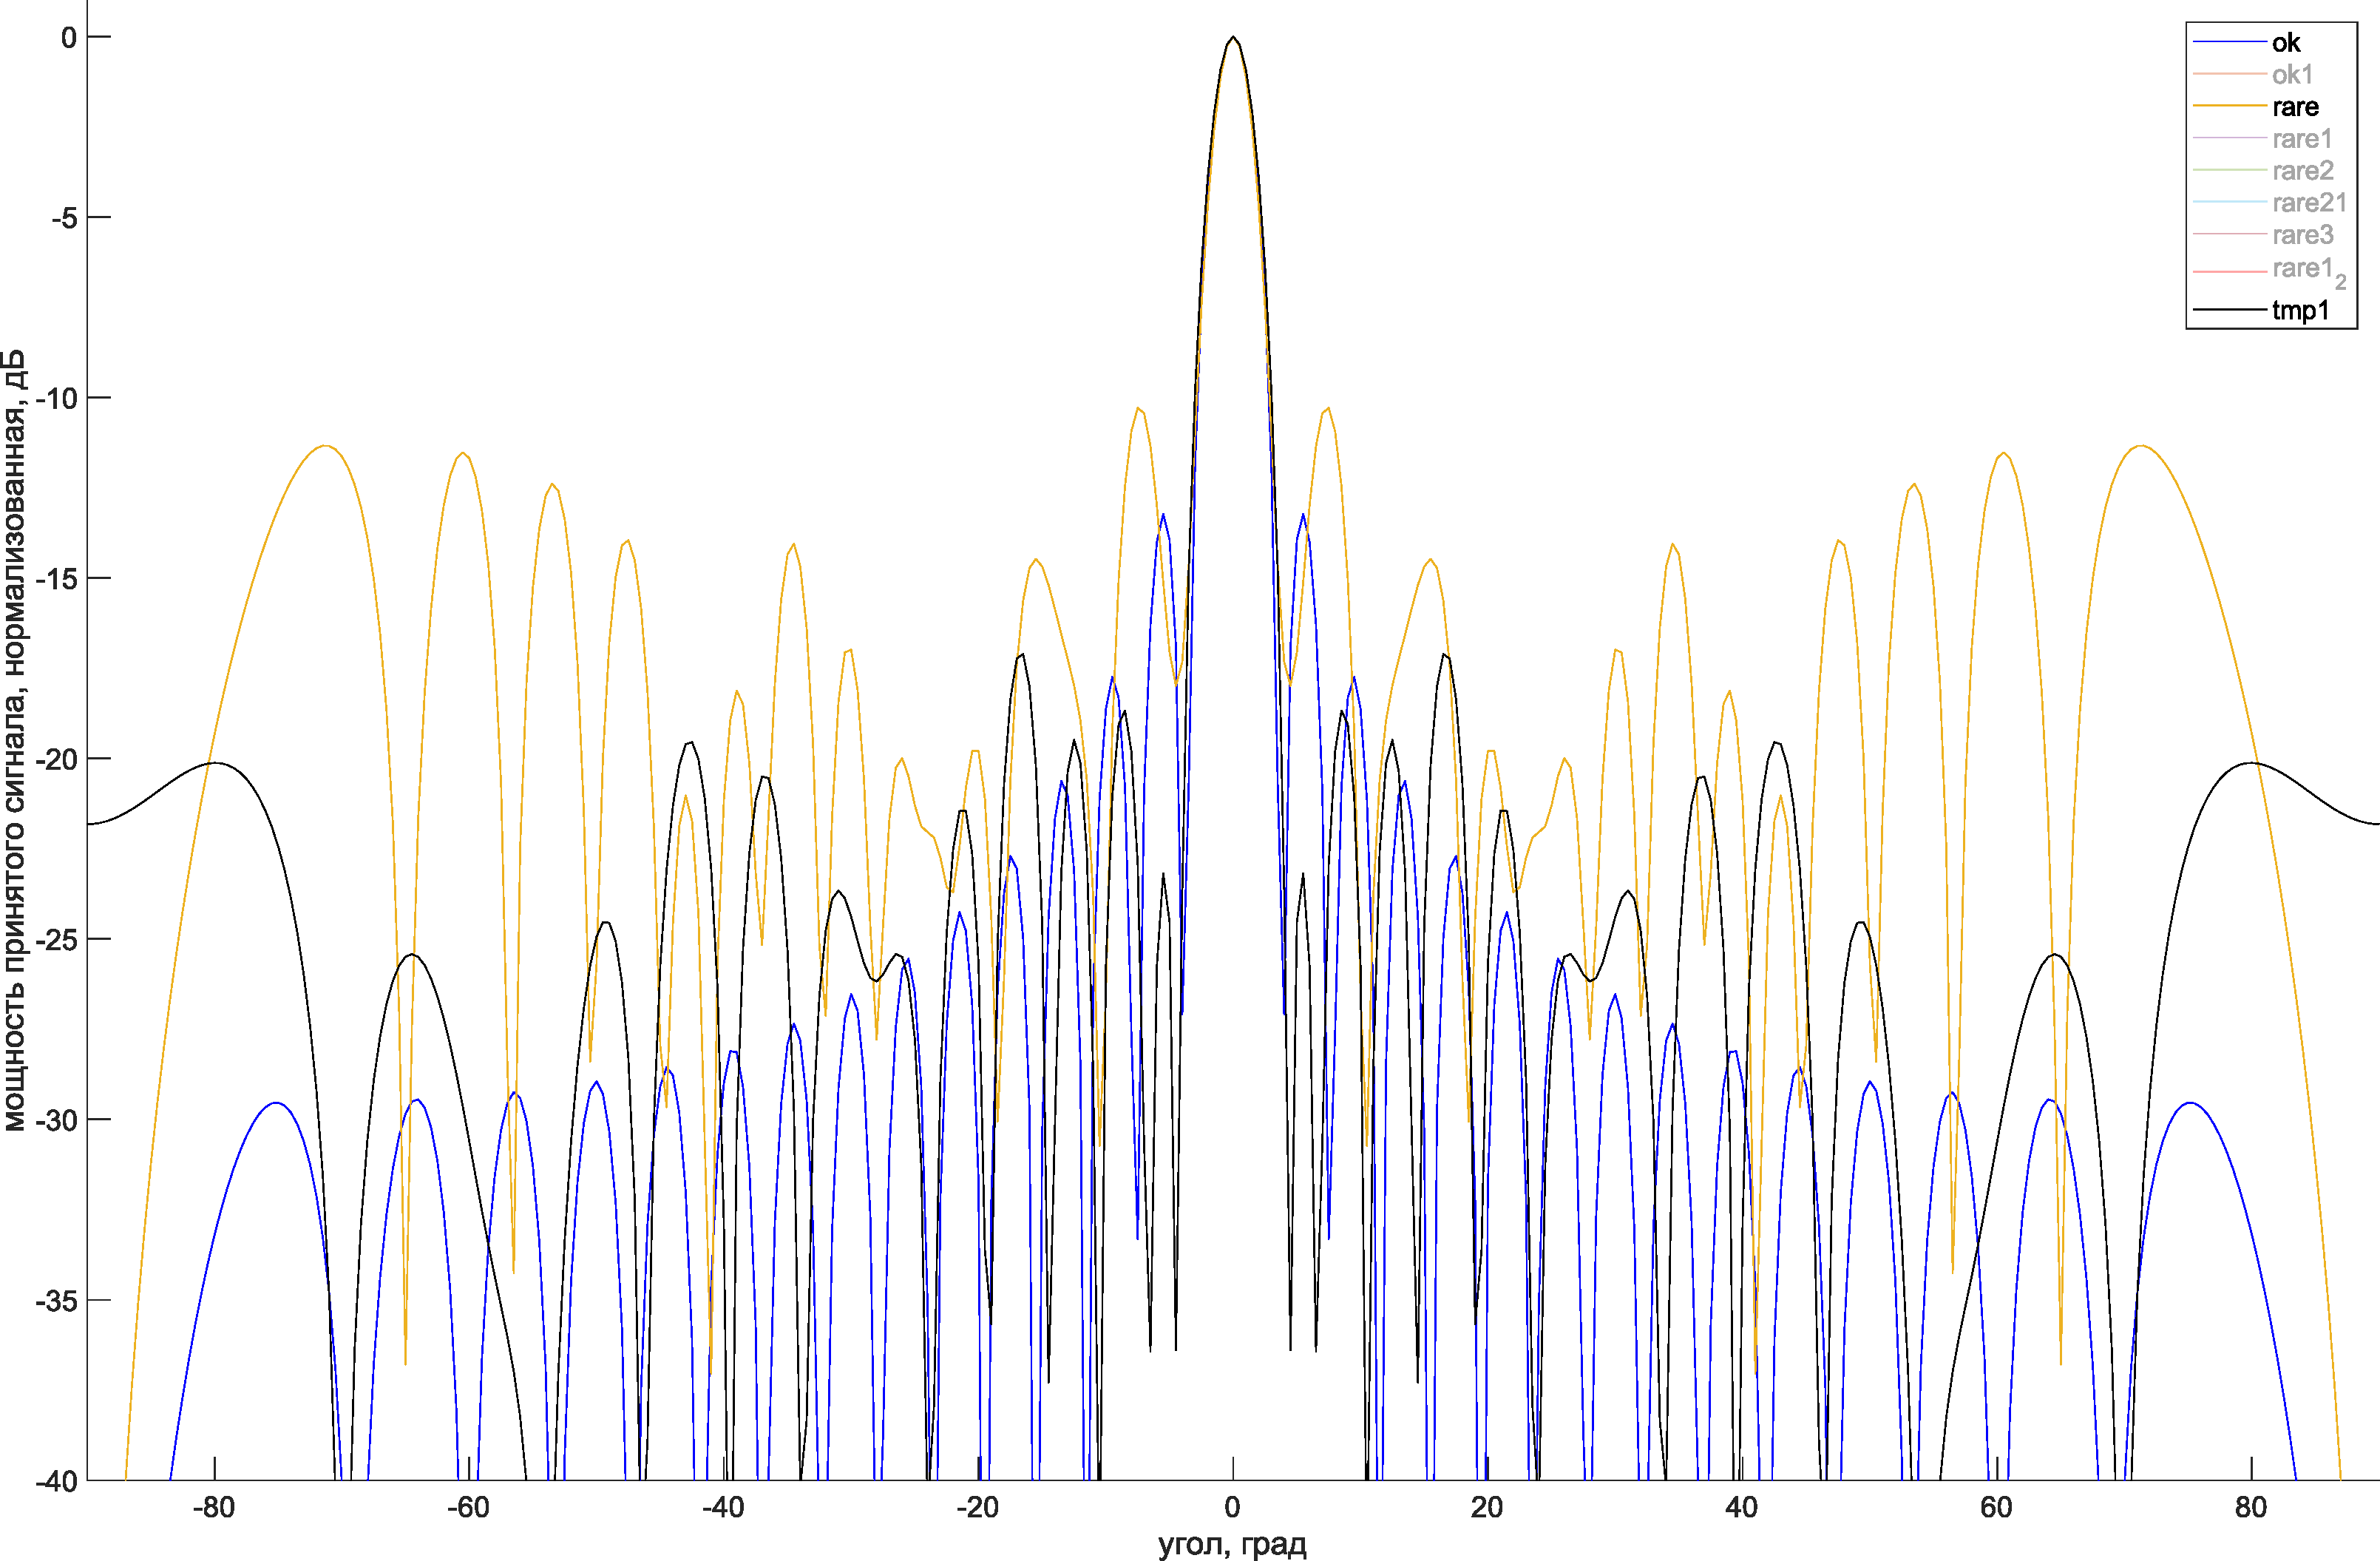
\includegraphics[width=0.8\textwidth,height=0.35\textheight,keepaspectratio]{iterative-array-raw-beam-pattern}
    \caption{Сравнение пространственных откликов от 
    (синий) эквидистантной решётки из 30 элементов
    (жёлтый) разреженной решётки из данного метода
    (чёрный) разреженной решётки с расширяющимся к краям распределением, сформированным по методике из раздела~\ref{sec:perturbations-method}
    }%
    \label{fig:iterative-array-raw-beam-pattern}
\end{figure}

Сравним данные результаты с результатами полученными методом итеративной обработки данных. Результат показан на Рисунке~\ref{fig:iterative-array-processed-beam-pattern}. 
Диаграмма направленности, полученная в результате применения данного метода, имеет меньший уровень боковых лепестков чем у равномерного и классического неравномерного распределений при той же ширине главного лепестка.Дифракционные лепестки также на низком уровне. 

\begin{figure}[H]
    \centering
    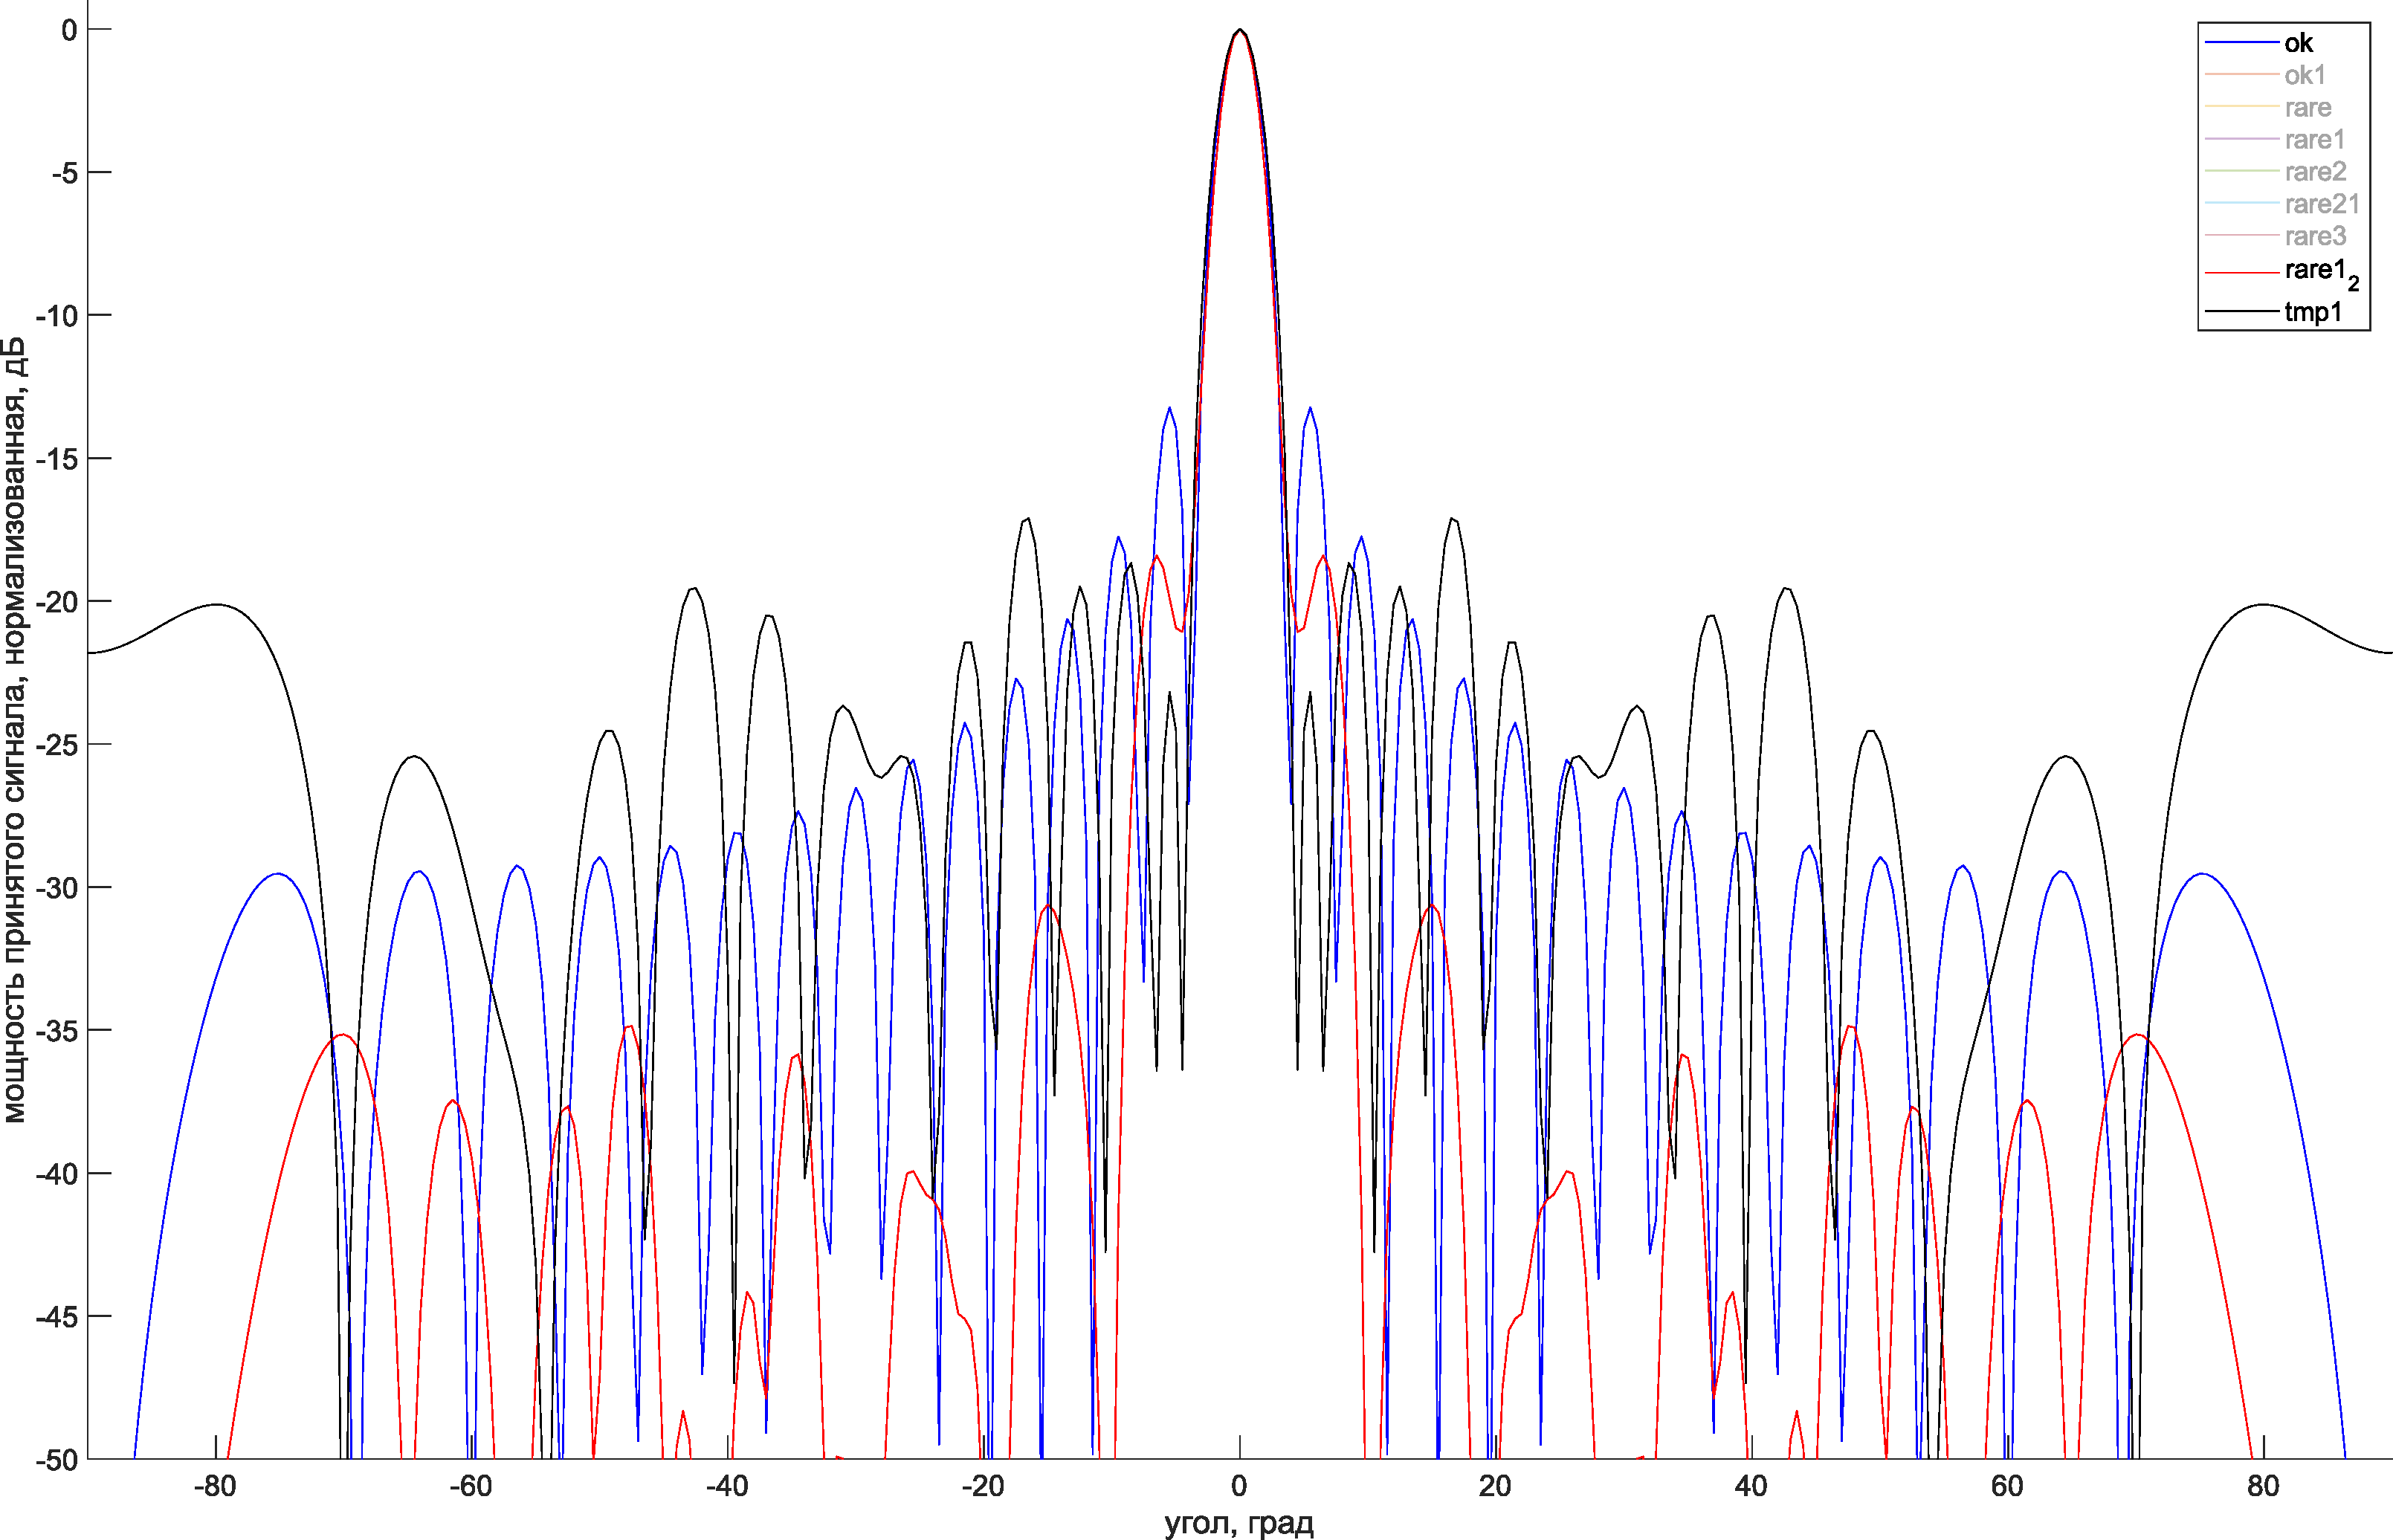
\includegraphics[width=0.8\textwidth,height=0.35\textheight,keepaspectratio]{iterative-array-processed-beam-pattern}
    \caption{Сравнение пространственных откликов от 
    (синий) эквидистантной решётки из 30 элементов
    (красный) синтезированной решётки из данного метода
    (чёрный) разреженной решётки с расширяющимся к краям распределением, сформированным по методике из раздела~\ref{sec:perturbations-method}
    }%
    \label{fig:iterative-array-processed-beam-pattern}
\end{figure}

Рассмотрим также следующую демосцену: зададим 4 сигнала с разной амплитудой

\begin{minted}[
    linenos,
    breaklines,
    frame=single,
    framesep=10pt
]{matlab}
aimAngles = [0 -20 30 50];
aimAmps   = [0 -1 -4 -2];
\end{minted}

Результат показан на Рисунке~\ref{fig:iterative-array-demo}

\begin{figure}[!ht]
    \centering
    \includegraphics[width=0.8\textwidth,height=0.35\textheight,keepaspectratio]{iterative-array-demo}
    \caption{ Сравнение пространственного отклика для 3 решёток}%
    \label{fig:iterative-array-demo}
\end{figure}

Видно, что у разреженной решётки ниже уровень боковых лепестков, однако на большом количестве целей чётко 
<<вылезли>> дифракционные лепестки слева, в то время у АР синтезированной методом итераций, 
дифракционные лепестки имеют низкий уровень. 

В то же время обнаруживается проблема, связанная с тем, как в рассматриваемом методе объединяются данные 
от разных подрешёток -- сигнал, который на 4~дБ слабее других сигналов в рамках того же отсчёта по 
дальности, оказался подавлен на ещё 3~дБ. Можно избавиться от этой проблемы если использовать 
более интеллектуальные алгоритмы объединения результатов, однако это является 
темой дальнейших исследований и не рассматривается в данной работе.

\subsection{Заключение}

Данный подход использует возможности ЦАР по раздельной обработке данных из каждого канала. 
Он имеет следующие преимущества:

\begin{itemize}
    \item Алгоритм интуитивно понятен и легко воспроизводим
    \item Подавление боковых лепестков -- такой подход позволяет добиться меньшего уровня боковых лепестков чем массив с 
    равномерным расположением элементов и чем у разреженной решётки с расширяющимся к краям распределением
    \item Уменьшение количества -- в показанном примере в разреженной решетке на $33,33$\% элементов 
    меньше чем в эквидистантной
\end{itemize}

Однако он в то же время обладает следующими недостатками:

\begin{itemize}
    \item Сложность вычислений:
    \begin{itemize}
        \item неравномерное расположение элементов не позволяет использовать быстрое 
        преобразование Фурье для диаграммообразования
        \item так как одни и те же данные используются несколько раз для расчёта результатов для одного отсчёта по 
        дальности, то увеличивается время обработки одного отсчёта и усложняется 
        проектирование вычислительного конвейера
    \end{itemize}
    \item Подавление слабых сигналов - если в рамках одного отсчёта по дальности в области обзора находится несколько 
    источников с сильно отличающимся уровнями сигналов, то более слабые сигналы могут быть подавлены, и источник останется 
    незамеченной, что является серьезным недостатком в ряде применений, особенно в военной промышленности. Однако данный 
    недостаток может быть устранён, если применять иной, отличный от прямого перемножения, способ объединения результатов.
\end{itemize}

В целом, данный подход имеет перспективы, однако метод объединения результатов нуждается 
в усовершенствовании и проведении дальнейших исследований. 


\section{Моделирование применения интерполяции для улучшения характеристик ДН}\label{sect:interpolation-modeling}

Рассмотрим разреженную эквидистантную решётку с межэлементным расстоянием $\lambda/1,4$. 
Для сравнения зададим эквидистантную решётку с межэлементным расстоянием $\lambda/2$. Также для более 
наглядной визуализации сигнала зададим решётку с шагом $\lambda/32$.

\begin{minted}[
    linenos,
    breaklines,
    frame=single,
    framesep=10pt
]{matlab}
f = 5e9; % 5 GHz
lam = freq2wavelen(f); % длина волны
% array params
xmtmin = -0;xmtmax = 12; % начальный и конечный безразмерные координаты элементов эквидистантной решётки с шагом lam/2
dOk = lam/2; % достаточное межэлементное расстояние
dNOk = lam/1.4; % МЭР для разреженной решётки
dSmooth = lam/32; % шаг для сглаживания и визуализации

dxOk = dOk*(xmtmin:1:xmtmax)'; % координаты элементов
NNOk = ceil((max(dxOk)-min(dxOk))/dNOk); % число элементов разреженной решётки
Nsmooth = ceil((max(dxOk)-min(dxOk))/dSmooth); % число элементов решётки для отображения

dxNOk = linspace(min(dxOk),max(dxOk),NNOk)';
dxSmooth = linspace(min(dxOk),max(dxOk),Nsmooth)';
\end{minted}

Если решётка принимает сигнал с направлений близких к направлению на 0~градусов, то значения сигналов не 
сильно отличаются друг от друга, и потому нельзя корректно оценить работу функции интерполяции. 
Проведём начальное исследование с направлением прихода сигнала $\theta=30$~градусов от нормали к плоскости АР. 
Разрешение пространственного отклика АР установим в {0,1}~градус.

\begin{minted}[
    linenos,
    breaklines,
    frame=single,
    framesep=10pt
]{matlab}
aimAngles = [30];
aimAmps   = [0]; %dB
resolution = 0.1; %deg
\end{minted}

Рассмотрим пространственный отклик, полученный для эквидистантных решёток на 
Рисунке~\ref{fig:interpolation-equally-spaced-modeling}.
Наблюдаем главный лепесток на 30~градусах. 
У разреженной решётки также виден дифракционный лепесток на -56~градусах.


\begin{figure}[H]
    \centering
    \begin{subfigure}[b]{0.49\textwidth}
        \centering
        \hspace*{-3ex}
        \includegraphics[width=\textwidth]{interpolation-equally-spaced-2}
        \caption{}%
    \end{subfigure}
    \hfill
    \begin{subfigure}[b]{0.49\textwidth}
        \centering
        \hspace*{-3ex}
        \includegraphics[width=\textwidth]{interpolation-equally-spaced-14}
        \caption{}%
    \end{subfigure}
    \caption{%
    Пространственный отклик эквидистантных решёток с шагом (а) $\lambda/2$ и (б)$\lambda/1,4$
    }%
    \label{fig:interpolation-equally-spaced-modeling}
\end{figure}

Отобразим распределение сигналов для эквидистантных решёток. Также добавим на рисунок графики двух 
сглаженных сигналов, полученных на решётке с шагом $d=\lambda/32$ с направлений +30 и -56~градусов. 
Результат показан на Рисунке~\ref{fig:interpolation-equally-spaced-values}. 

\begin{figure}[H]
    \centering
    \includegraphics[width=0.8\textwidth]{interpolation-equally-spaced-values}
    \caption{Cравнение распределений для сигналов от целей на +30 и на -56
    градусов от нормали к плоскости антенной решётки}
    \label{fig:interpolation-equally-spaced-values}
\end{figure}

Видно, что значения сигнала на разреженной решётке попадают на пересечения распределений от 
источников на +30 и -56~градусов. Соответственно, в данном случае информация от 
них неотличима, и её не получится использовать для интерполяции.

Создадим ещё одну разреженную решётку с количеством элементов как в эквидистантной разреженной решётке, 
однако с неэквидистантным расположением элементов. При таком расположении элементов информация, 
получаемая при приёме сигналов с различных направлений всегда будет отличаться.

\begin{minted}[
    linenos,
    breaklines,
    frame=single,
    framesep=10pt
]{matlab}
deltas = [0.9 2 1.1 1];
half = cumsum(deltas);
rare2 = dOk*(max(half)+[fliplr(-half),0,half])';
\end{minted}

\begin{figure}[H]
    \centering
    \includegraphics[width=0.8\textwidth]{interpolation-array-pos}
    \caption{Иллюстрация расположения элементов в разреженной решётке}
    \label{fig:interpolation-array-pos}
\end{figure}
    

Расположение выбрано для соответствия поведению функции interp1 из пакета MATLAB: 
Функция interp1 проводит интерполяцию данных в одномерном массиве принимая на вход исходные данные и сетку, 
в которой они расположены, и пересчитывает значения для выходной сетки, используя значения из N ближайших точек 
исходной сетки. 
В данном распределении единичные участки с межэлементным расстоянием $d\gg\lambda/2$ находятся между 
групп элементов с шагом $d\leq \lambda/2$;
значения из узлов с более плотным расположением элементов будут использованы для вычисления значений виртуальных 
элементов в участках с большим межэлементным расстоянием. 

Для неравномерной сетки применимы следующие методы функции interp1:

\begin{itemize}
    \item pchip -- требует минимум 4 точки, кубическая интерполяция
    \item makima -- требует минимум 2 точки, модифицированная кубическая Эрмитова интерполяция
    \item spline -- требует минимум 4 точки, сплайн интерполяция
\end{itemize}

На Рисунке~\ref{fig:interpolation-values-interp-30} показаны результаты интерполяции с применением метода spline. 
Интерполированные данные показаны 
точками синего цвета. Пространственный отклик для интерполированной решётки показан на 
Рисунке~\ref{fig:interpolation-processed-pattern-30}. 
Видно, что при применении интерполяции уровень дифракционных лепестков меньше на {3,5}~дБ по сравнению 
с исходной решёткой без применения интерполяции и на 15~дБ меньше чем в 
эквидистантной разреженной решётке.

\begin{figure}[H]
    \centering
    \includegraphics[width=0.8\textwidth]{interpolation-values-interp-30}
    \caption{Сравнение распределений сигналов на различных АР}
    \label{fig:interpolation-values-interp-30}
\end{figure}

\begin{figure}[H]
    \centering
    \begin{subfigure}[b]{0.49\textwidth}
        \centering
        \hspace*{-3ex}
        \includegraphics[width=\textwidth]{interpolation-raw-pattern-30}
        \caption{}%
    \end{subfigure}
    \hfill
    \begin{subfigure}[b]{0.49\textwidth}
        \centering
        \hspace*{-3ex}
        \includegraphics[width=\textwidth]{interpolation-processed-pattern-30}
        \caption{}%
        \label{fig:interpolation-processed-pattern-30}
    \end{subfigure}
    \caption{%
    (а) ДН разреженной решётки
    (б) ДН интерполированной решётки
    }%
    \label{fig:interpolation-pattern-30}
\end{figure}

Проведём ещё одно исследование: увеличим угол отклонения цели от нормального направления до 50 градусов. 
Как видно на Рисунке \ref{fig:interpolation-processed-pattern-50}, применение интерполяции в данном случае 
привело к обратному результату -- в диаграмме направленности лишь усилились нежелательные составляющие. 

\begin{figure}[H]
    \centering
    \begin{subfigure}[b]{0.49\textwidth}
        \centering
        \hspace*{-3ex}
        \includegraphics[width=\textwidth]{interpolation-raw-pattern-50}
        \caption{}%
    \end{subfigure}
    \hfill
    \begin{subfigure}[b]{0.49\textwidth}
        \centering
        \hspace*{-3ex}
        \includegraphics[width=\textwidth]{interpolation-processed-pattern-50}
        \caption{}%
        \label{fig:interpolation-processed-pattern-50}
    \end{subfigure}
    \caption{%
    (а) ДН разреженной решётки
    (б) ДН интерполированной решётки
    }%
    \label{fig:interpolation-pattern-50}
\end{figure}

Рассмотрим распределение сигнала на элементах:

\begin{figure}[H]
    \centering
    \includegraphics[width=0.8\textwidth]{interpolation-values-interp-50}
    \caption{Сравнение распределений сигналов на различных АР}
    \label{fig:interpolation-values-interp-50}
\end{figure}


Видим, что интерполированные значения сильно отличаются от идеальных т.к. амплитуда колебаний сплайн функции 
меньше амплитуды колебаний синусоидального сигнала. Выбранный метод интерполяции 
плохо подходит для восстановления сигнала. Однако возможно несколько вариантов решения задачи:

\begin{itemize}
    \item Увеличение порядка интерполирующего многочлена для использования большего числа окружающих 
    точек для вычислений, и применение их к АР c большим числом элементов
    \item Применение другого способа интерполяции, учитывающего периодичность сигналов, 
    и использующего все доступные элементы для вычислений каждого значения
\end{itemize}

Оба варианта требуют более глубокого изучения численных методов математического анализа и 
являются темами для дальнейших исследований данного метода.


\subsection{Заключение}

Недостаток данного подхода такой же как у всех других, основанных на применении цифровых антенных решеток, 
а именно -- сложность вычислений. Каждый отсчёт по дальности необходимо дополнительно обрабатывать для 
получения интерполированных распределений, что требует либо применения более производительных центральных процессоров 
либо построения более эффективной параллельной конвейерной архитектуры. Данный недостаток будет всё сильнее проявляться 
с увеличением размера исходной цифровой решётки. В то же время, вычисление значений с помощью интерполяции требует 
меньшего числа операций чем свёртка, которая применяется при поканальной обработке сигнала по дальности. 
Так как данный метод предполагает уменьшение числа элементов антенной решётки, то возможно 
также и уменьшение количества выполняемых операций.

Среди предполагаемых достоинств данного метода можно выделить следующие:

\begin{itemize}
    \item Подавление боковых лепестков - такой подход позволяет добиться меньшего уровня боковых лепестков чем при 
    использовании эквидистантных и неэквидистантных решёток при том же количестве антенных элементов
    \item Экономия средств - как и предыдущий метод, данный позволит уменьшить число антенных элементов по сравнению с 
    эквидистантными ЦАР при схожих параметрах диаграмм направленности.
    \item Выравнивание вычислительной сетки - выходными данными подпрограммы интерполяции являются значения сигналов на 
    виртуальной эквидистантной решётке, что может позволить применять БПФ для ускорения построения ДН, что важно для 
    многолучевых АР и алгоритмов определения направления прихода сигнала. 
\end{itemize}

В целом, стоит отметить, что данный метод выглядит перспективным, однако требует проведения дополнительных исследований. 
Возможно, при использовании данного подхода для каждой конкретной задачи потребуется 
проводить большое количество вычислений для поиска оптимальных распределений для лучших результатов интерполяции. 


\section{Моделирование когерентного MIMO радиолокатора}\label{sect:mimo-modeling}

Рассмотрим структуру модели MIMO радиолокатора второго вида (по классификации из \cite{li2008mimo}),
также называемого когерентным MIMO радаром.

Модель проводит симуляцию для $N$ передающих элементов расположенных линейно вдоль оси
$Ox$ и $M$ приёмных, расположенных вдоль оси $Oy$.

\begin{figure}[H]
    \centering
    \begin{subfigure}[b]{0.49\textwidth}
        \centering
        \hspace*{-3ex}
        \includegraphics[width=\textwidth]{MIMO-TX}
        \caption{}%
    \end{subfigure}
    \hfill
    \begin{subfigure}[b]{0.49\textwidth}
        \centering
        \hspace*{-3ex}
        \includegraphics[width=\textwidth]{MIMO-RX}
        \caption{}%
    \end{subfigure}
    \caption{положения антенных элементов}%
    \label{fig:mimo-elemnt-pos}
\end{figure}


В результате совместной обработки будет получена виртуальная решётка, показанная на Рисунке~\ref{fig:mimo-virtual-array}.

\begin{figure}[H]
    \centering
    \includegraphics[width=0.8\textwidth,height=0.35\textheight,keepaspectratio]{MIMO-Virtual}
    \caption{Геометрия синтезированной антенной решётки. Виртуальные элементы отмечены серым цветом}%
    \label{fig:mimo-virtual-array}
\end{figure}

Входными данными в программу симуляции являются координаты цели в сферических координатах
с началом в центре виртуальной решётки.

В Таблице~\ref{table:mimo-model-parameters} приведены параметры целей, которые будут обнаруживаться в процессе симуляции.


\begin{table}[H]
    \centering
    \begin{tabular}{|c|c|c|}
        \hline
        $R$, м & $\theta$, град & $\phi$, град \\ \hline
        1500   & 20             & 25           \\ \hline
        1000   & -20            & -25          \\ \hline
    \end{tabular}
    \caption{Параметры целей}\label{table:mimo-model-parameters}
\end{table}

Работа программы моделирования состоит из следующих этапов:

\begin{enumerate}
    \item Задание параметров АР
    \item Генерация М-последовательностей для каждого элемента передающей решётки. 
    \item Модуляция передаваемых сигналом с помощью BPSK. Модуляция происходит с помощью комплексной экспоненты на нулевой частоте.
    \item Расчёт сигналов, излучаемых передающей решёткой и принятых на i-той цели
    \item Расчёт и сложение комплексных сигналов, отражённых от целей, и принятых на приёмной решётке
    \item Проведение свёртки по дальности для каждой отдельной M-последовательности. Формирование виртуальной АР
    \item Расчёт ДН для каждой дальности
    \item Обработка ДН, удаление сигналов меньше определённой амплитуды
    \item Сведение всех дальностей в общую плоскость решений
\end{enumerate}

Результат работы программы показан на Рисунке \ref{fig:mimo-modeling-result}. 
Исходный код программы приведён в Приложении \ref{appendix:mimo-modeling-appendix}.


\begin{figure}[H]
    \centering
    \includegraphics[width=0.8\textwidth,height=0.4\textheight,keepaspectratio]{mimo-modeling-result}
    \caption{Результаты моделирования MIMO радиолокатора}%
    \label{fig:mimo-modeling-result}
\end{figure}

\subsection{Заключение}

MIMO радиолокаторы обладают следующими преимуществами:

\begin{itemize}
    \item Компактность -- антенны MIMO радаров обладают меньшими размерами по сравнению с классическими АФАР,
    ввиду меньшего количества антенных элементов 
    \item Адаптивная цифровая обработка -- так как все вычисления проходят в цифровой части радиолокатора, 
    адаптивная обработка сигналов, в частности, подавление помех и формирование сложных ДНА, 
    может быть выполнена более качественно. 
    \item Увеличение угловой разрешающей способности -- возможности ЦАР по формировании более подходящих 
    для данных задач коэффициентов, позволяет MIMO радиолокаторам достигать 
    более высокой разрешающей способности по сравнению с классическими АФАР и SIMO радарами с тем же количеством элементов.
    \item Увеличение разрешающей способности и чувствительности при детектировании движущихся целей -- 
    MIMO радары лучше обнаруживают медленно движущиеся цели, чем классические АФАР с тем же количеством элементов
    \item Реконфигурируемость -- технические характеристики MIMO радаров связаны с возможностями обрабатывающей 
    техники. Вычислительные процессоры совершенствуются каждый год, 
    предлагая увеличение производительности от 10~до~50\% по сравнению с прошлыми реализациями. 
    Улучшить возможности MIMO радаров по формированию многолучевых ДН, активному сопровождению целей и 
    идентификации направления прихода сигнала можно за счёт обновления только системы обработки, 
    тогда как более дорогая аналоговая часть будет оставаться неизменной
\end{itemize}

В то же время они обладают следующими недостатками:

\begin{itemize}
    \item Сложность проектирования систем обработки -- MIMO радары генерируют большое количество данных. 
    Необходимо успевать обрабатывать текущий набор данных до того как придёт следующий, 
    что требует проектирования более сложной программной архитектуры и 
    параллельных цифровых аппаратных обработчиков данных
    \item Синхронизация между каналами -- для эффективной работы радара необходимо очень точно 
    синхронизировать тактовые сигналы как между каналами одного типа, 
    так и между приёмниками и передатчиками. 
    Влияние рассинхронизации на точность результатов подробно описаны в работе \cite{bondarenko2011affection}.
    \item Сложность детектирования быстродвижущихся целей
\end{itemize}

Тем не менее, исследования MIMO радаров активно ведутся, предлагая новые, более эффективные архитектуры и 
методы обработки сигналов. 
На текущий момент MIMO радары являются передовой областью в радарной технике. 
Однако их повсеместное внедрение связано с рядом технических и практических вызовов: сложность и стоимость таких систем,
требования к энергопотреблению и необходимость проектирования 
мощных систем обработки принятых данных являются преградами к их применению. 

Таким образом можно заключить, что MIMO радары обладают большим потенциалом, 
однако их массовое внедрение может произойти только по прошествию 
нескольких лет развития современной вычислительной техники.

\ssect{Итоги исследования}\label{chap:conclusions}

В данной магистерской диссертации были рассмотрены различные аспекты проектирования и функционирования современных 
антенных решёток и радиолокационных систем. Исследование охватило несколько тем, начиная от методов 
применимым к классическим антенным решёткам - неравномерные амплитудные распределения, 
проектирование неэквидистантных антенных решёток; 
и заканчивая рядом методов применимым к современным цифровым антенным решёткам. 

В ходе выполнения работы были решены следующие задачи

\begin{enumerate}
    \item Рассмотрены методы формирования неравномерных амплитудных распределений, 
    проведено моделирование и сравнение результатов
    \item Изучены методы проектирования антенных решёток с непостоянным межэлементным расстоянием. 
    Проведено их сравнение, описаны возможности и особенности их эффективного применения для различных задач. 
    Проведено моделирование и сравнение результатов. Сделаны выводы по разработанным моделям.
    \item Изучен метод итеративной обработки данных при диаграммообразовании в цифровых антенных решётках. 
    Приведены достоинства и недостатки метода. 
    Указаны возможности для дальнейших исследований и пути развития.
    \item Рассмотрено применение MIMO радиолокаторов. 
    Проведено моделирование когерентного MIMO радара. 
    Изучены практические и теоретические аспекты их применения в радиолокации. 
    Приведены достоинства и недостатки. 
    Сделаны выводы по возможностям их использования в современных системах.
\end{enumerate}

Результатом данной работы является разработанный набор моделей, 
которые могут быть использованы в дальнейших исследованиях и в рабочих процессах 
при выборе типа и проектировании антенных решёток. 



\nocite{*}
\printbibliography[title={Список использованных источников},heading=bibintoc]
% \appendix
% \section{Листинг кода программы моделирования АР.}%
\label{appendix:arrays-code-appendix}

\begin{minted}[
    linenos,
    breaklines,
    frame=single,
    framesep=10pt,
    fontsize=\small
]{matlab}
function [distributionValues,phases] = distribution_former(dx,f, phi,amp_dB)
if(size(phi) ~= size(amp_dB))
    error("sizes unequal")
end

amp = db2pow(amp_dB);
distributionValues = zeros(size(dx));
phases = zeros(length(dx),length(phi));
for ind = 1:length(phi)
phases(:,ind) = 2.*pi.*f.*dx.*sind(phi(ind)) /physconst("Lightspeed");
distributionValues = distributionValues + amp(ind).*exp(1i.*phases(:,ind));
end
end    
\end{minted}


\begin{minted}[
    linenos,
    breaklines,
    frame=single,
    framesep=10pt,
    fontsize=\small
]{matlab}
function [channel_res,theta] = aec_simulation(dVals,dx,f, resolution, theta)
if nargin < 4
    resolution = 0.5;
end
if nargin < 5
    theta = (-90:resolution:90);
end
channel_coeff = exp(1i.* (-2.*pi.*f.*dx.*sind(theta) /physconst("Lightspeed")));
channel_res = sum(dVals.*channel_coeff,1);
end 
\end{minted}
\appendix
\renewcommand{\thesection}{\Asbuk{section}} % To use Cyrillic letters for appendix sections
\titleformat{\section}[block]{\Large\normalfont\bfseries\raggedright}{\appendixname\ \thesection.}{1ex}{}
\section{Листинг кода программы моделирования АР.}%
\label{appendix:arrays-code-appendix}

\begin{minted}[
    linenos,
    breaklines,
    frame=single,
    framesep=10pt,
    fontsize=\small
]{matlab}
function [distributionValues,phases] = distribution_former(dx,f, phi,amp_dB)
if(size(phi) ~= size(amp_dB))
    error("sizes unequal")
end

amp = db2pow(amp_dB);
distributionValues = zeros(size(dx));
phases = zeros(length(dx),length(phi));
for ind = 1:length(phi)
phases(:,ind) = 2.*pi.*f.*dx.*sind(phi(ind)) /physconst("Lightspeed");
distributionValues = distributionValues + amp(ind).*exp(1i.*phases(:,ind));
end
end    
\end{minted}


\begin{minted}[
    linenos,
    breaklines,
    frame=single,
    framesep=10pt,
    fontsize=\small
]{matlab}
function [channel_res,theta] = aec_simulation(dVals,dx,f, resolution, theta)
if nargin < 4
    resolution = 0.5;
end
if nargin < 5
    theta = (-90:resolution:90);
end
channel_coeff = exp(1i.* (-2.*pi.*f.*dx.*sind(theta) /physconst("Lightspeed")));
channel_res = sum(dVals.*channel_coeff,1);
end 
\end{minted}
\section{Листинг кода программы моделирования когерентного MIMO радиолокатора.}%
\label{appendix:mimo-modeling-appendix}

\inputminted[
    linenos,
    breaklines,
    frame=single,
    framesep=10pt,
    fontsize=\small
]{matlab}{code/mimo_model.m}



\end{document}